
%!TEX option = --shell-escape

\documentclass[9pt, xcolor={svgnames, x11names},professionalfonts]{beamer}


% \usetikzlibrary{decorations.markings, decorations.fractals}
% \usetikzlibrary{shapes.callouts,shapes.multipart}
% \usetikzlibrary{positioning}

% \setlength{\TPHorizModule}{1.0cm}
% \setlength{\TPVertModule}{\TPHorizModule}

\usepackage{xcolor}
\usepackage{cancel}
\usepackage{bm}
\usepackage{graphicx}
\usepackage[x11names, svgnames]{xcolor} % for colors in handouts, auto loaded in Beamer?
\usepackage{tikz}
\usetikzlibrary{arrows.meta, math, calc, shadows}
\usetikzlibrary{decorations.markings, decorations.fractals, decorations.text} % for chain, etc.
\usetikzlibrary{intersections}
\usepackage{pgfmath}
\usepackage{ifthen}
\usepgfmodule{oo}
\usepgflibrary{shadings}
% \usetikzlibrary{decorations.shapes}
\usepackage[many]{tcolorbox}
\usepackage[absolute,overlay,showboxes]{textpos}
% \usepackage{textpos}
% \textblockorigin{0.0cm}{0.0cm}  %start all at upper left corner
\TPshowboxesfalse

\newcommand\lb{\linebreak}
\newcommand\Ra{\Rightarrow}
\newcommand\cd{\!\cdot\!}
\newcommand\x{\!\times\!}
\newcommand\pars{\par\smallskip}
\newcommand\parm{\par\medskip}
\newcommand\parb{\par\bigskip}
\renewcommand{\deg}{^\circ}

% counter for resuming enumerated list numbers
\newcounter{resumeenumi}
\newcommand{\suspend}{\setcounter{resumeenumi}{\theenumi}}
\newcommand{\resume}{\setcounter{enumi}{\theresumeenumi}}



% https://tex.stackexchange.com/questions/33703/extract-x-y-coordinate-of-an-arbitrary-point-in-tikz
\makeatletter
\providecommand{\gettikzxy}[3]{%
	\tikz@scan@one@point\pgfutil@firstofone#1\relax
	\edef#2{\the\pgf@x}%
	\edef#3{\the\pgf@y}%
}
\makeatother

\makeatletter
\newcommand{\verbatimfont}[1]{\def\verbatim@font{#1}}%
\makeatother

%%%%%%%%%%%%%%%%%%%%%%%%%%%%%%%%%%%%%%%%%%%%%%%%%%%%%%%%%%%%%%%%%%%%%%%%%%%%%%%%


\newcommand{\tb}[4][0.8]{
	\begin{textblock*}{#1}(#2, #3)
		% \raggedright
		#4
	\end{textblock*}
}

\newtcolorbox{statsbox}[2][] { 
  colback=white,
  colbacktitle=structure,
  colframe=structure,
  coltitle=white,  
  top=0.25cm,
	bottom=0.125cm,
	left=0mm,
	right=0mm,
  % fonttitle=\itshape\rmfamily,
  halign=flush left, 
  enhanced,
  drop fuzzy shadow,
  attach boxed title to top left={xshift=3.5mm, yshift=-2mm},
  title={#2}, #1}
\newtcolorbox{redbox}{colback=white, colframe=structure, enhanced, drop fuzzy shadow}
\newtcolorbox{titledbox}[1]{colback=white,colframe=structure,title={#1}}
\newtcbox{\tcb}[1][]{colback=white,boxsep=0pt,top=5pt,bottom=5pt,left=5pt,
		right=5pt, colframe=structure,  enhanced, drop fuzzy shadow, #1}
% tcb title
\newtcbox{\tcbt}[2][]{colback=white,boxsep=0pt,top=5pt,bottom=5pt,left=5pt,
		right=5pt, colframe=structure, enhanced, drop fuzzy shadow,  title={#2}, #1}
% tcb left title
\newtcbox{\tcbtl}[2][]{ colback=white,
  colbacktitle=structure,
  colframe=structure,
  coltitle=white,  
  top=0.25cm,
	bottom=0.125cm,
	left=0mm,
	right=0mm,
  % fonttitle=\bfseries,
  halign=flush left, 
  enhanced,
  drop fuzzy shadow,
  attach boxed title to top left={xshift=3.5mm, yshift=-2mm}, 
	title={#2}, #1}

\newtcbtheorem{myexam}{Example}%
{
	enhanced,
	colback=white,
	colframe=structure,
	% fonttitle=\bfseries,
	fonttitle=\itshape\rmfamily,
	drop fuzzy shadow,
	%description font=\mdseries\itshape,
	attach boxed title to top left={yshift=-2mm, xshift=5mm},
	colbacktitle=structure
	}{exam}% then \pageref{exer:theoexample} references the theo

% \newcommand{\myexample}[2][red]{
% 	% \tcb\tcbset{theostyle/.style={colframe=red,colbacktitle=yellow}}
% 	\begin{myexam}{}{}
% 		#2
% 	\end{myexam}
% 	% \tcbset{colframe=structure,colbacktitle=structure}
% }

\newtcbtheorem{myexer}{Exercise}%
{
	enhanced,
	colback=white,
	colframe=structure,
	% fonttitle=\bfseries,
	drop fuzzy shadow,
	fonttitle=\itshape\rmfamily,
	% description font=\mdseries\itshape,
	attach boxed title to top left={yshift=-2mm, xshift=5mm},
	colbacktitle=structure
	}{exer}



\newcommand{\mini}[2][0.8]{
	\begin{minipage}[c]{#1\columnwidth}
		\raggedright
		#2
	\end{minipage}
}
\newcommand{\minit}[2][0.8]{
	\begin{minipage}[t]{#1\columnwidth}
		% \raggedright
		#2
	\end{minipage}
}

% centered minipage with text \raggedright
%\cmini[width]{content}
\newcommand{\cmini}[2][0.8]{
	\begin{center}
		\begin{minipage}{#1\columnwidth}
			\raggedright
			#2
		\end{minipage}
	\end{center}
}



\newcommand{\fig}[2][1]{% scaled graphic
	\includegraphics[scale=#1]{#2}
}

% centred framed colored box black border
%\cbox[width]{content}
\newcommand{\cbox}[2][1]{% framed centered color box
	\setlength\fboxsep{5mm}
	\setlength\fboxrule{.2 mm}
	\begin{center}
		\fcolorbox{black}{white}{
			\vspace{-0.5cm}
			\begin{minipage}{#1\columnwidth}
				\raggedright
				#2
			\end{minipage}
		}
	\end{center}
	\setlength\fboxsep{0cm}
}

\newcommand{\cfig}[2][1]{% centred, scaled graphic
	\begin{center}
		\includegraphics[scale=#1]{#2}
	\end{center}
}






 \definecolor{saitPurple}{RGB}{112,40,119}
 \definecolor{statsMaroon}{rgb}{0.55, 0, 0}
 \definecolor{saitMaroon}{rgb}{0.55, 0, 0}
 \definecolor{statsRed}{RGB}{224,38,37}
 \definecolor{saitRed}{RGB}{224,38,37}
 \definecolor{saitBlue}{rgb}{0, 0.59, 0.85}
 \definecolor{statsBlue}{rgb}{0, 0.59, 0.85}
 \definecolor{statsDeepBlue}{RGB}{0, 99, 167}
 \definecolor{saitDeepBlue}{RGB}{0, 99, 167}
 \definecolor{saitDeepBlue}{RGB}{0, 99, 167}
 \definecolor{LightGrey}{RGB}{200,200,200}
%  \definecolor{boxBG}{RGB}{236, 227, 227}
%  \definecolor{boxBG}{RGB}{242, 233, 223}
% !TEX root = ../Beamer/02ForceVectors/02ForceVectors.tex


\newcommand{\EyeBolt}[6][0]{
	\def\lrotate{#1};
	\def\lpin{#2}
	\def\lfill{#3}
	\def\ldraw{#4}
	\def\lscale{#5}
	\def\lwidth{#6}
	%\def\h{1.5}
	\def\r{0.3}
	\begin{scope}[scale=\lscale, rotate=\lrotate]
		\filldraw[draw=\ldraw, fill=\lfill, line width=\lwidth pt] ($(\lpin) + (-0.7,-1.25)$) arc(180:90:.2) -- ++(0.05,0)arc(-90:0:0.2) -- ++(0.05,0.65)arc(225:-45:0.28284)-- ++(0.05,-.65)arc(180:270:.2)-- ++(0.05,0)arc(90:0:0.2) -- cycle;
		\fill[outer color=\lfill, inner color=black, line width = 0] (\lpin) circle (2.25mm);
		\filldraw[fill=white, draw=\ldraw, line width = \lwidth pt] (\lpin) circle (1.25mm);

		\begin{scope}[even odd rule]
			\fill[\lfill] (\lpin) circle (2.5mm)
			(\lpin) circle (2.125mm);
		\end{scope}

		\filldraw[rounded corners=\lscale pt, draw=\ldraw, fill=\lfill, line width=\lwidth pt] ($ (\lpin) - (1,1.5) $) rectangle +(2,0.25);
	\end{scope}
}

% !TEX root = ../../Beamer/statikz/statikz.tex


\newcommand{\EyeConnection}[6][0]{
	\def\lrotate{#1};
	\def\lpin{#2}
	\def\lfill{#3}
	\def\ldraw{#4}
	\def\lscale{#5}
	\def\lwidth{#6}
	\def\h{1}
	\def\r{0.3}
	\begin{scope}[scale=\lscale, rotate=\lrotate]
		\filldraw[draw=\ldraw, fill=\lfill, line width=\lwidth pt] ($(\lpin) + (0.201*\h+1.0353*\r ,-0.75*\h)$) -- ++(105: 0.77646*\h+0.26795*\r) arc (15:165:\r) -- ++(-105:0.77646*\h+0.26795*\r) -- cycle;

		\fill[outer color=\lfill, middle color=red, inner color=black, line width = \lwidth pt] (\lpin) circle (2.5mm);
		\filldraw[fill=white, draw=\ldraw, line width = \lwidth pt] (\lpin) circle (1.25mm);

		\filldraw[rounded corners=\lscale pt, draw=\ldraw, fill=\lfill, line width=\lwidth pt] ($ (\lpin) - (1,1) $) rectangle +(2,0.25);
	\end{scope}
}

%\Member{startpt}{endpt}{outer fill color}{inner fill color}{stroke}{height}{radius}{linewidth}
\providecommand{\Member}[8]{
  % name the points
  \coordinate(start) at (#1);
  \coordinate(end) at (#2);
  \edef\ofill{#3}%
  \edef\ifill{#4}%
  \edef\stroke{#5}%
  \edef\height{#6} % cm
  \edef\radius{#7} % cm
  \edef\linewidth{#8} % mm

  \coordinate(delta) at ($ (end)-(start) $);
  \gettikzxy{(delta)}{\dx}{\dy}
  \gettikzxy{(start)}{\sx}{\sy}
  \pgfmathparse{veclen(\dx, \dy)} \let\length\pgfmathresult

  \pgfmathparse{\dx==0}%
  % \ifnum low-level TeX for integers
  \ifnum\pgfmathresult=1 % \dx == 0
    \pgfmathsetmacro{\rot}{\dy > 0 ? 90 : -90}
  \else
    \pgfmathsetmacro{\rot}{\dx > 0 ? atan(\dy / \dx) : 180 + atan(\dy / \dx)}
  \fi

  
   
  \shadedraw[transform canvas = { rotate around = {\rot:(\sx,\sy)}}, line width = \linewidth, rounded corners = \radius mm, top color = \ofill, bottom color = \ofill, middle color = \ifill, draw = \stroke] ($ (start)+(-0.5*\height, 0.5*\height) $) -- ++(\height cm +\length pt, 0 ) -- ++(0, -\height) -- ++ (-\height cm -\length pt, 0) -- cycle;


  \shadedraw[ball color = \ofill!50!\ifill, draw = \stroke] (start) circle (\height/8);
  \shadedraw[ball color = \ofill!50!\ifill, draw = \stroke] (end) circle (\height/8);
  %  \pgfresetboundingbox

  
  


}


\newcommand{\PC}[6][0]{%
  \edef\lrotate{#1}%
  \edef\lpin{#2}%
  \edef\lfill{#3}%
  \edef\ldraw{#4}%
  \edef\lscale{#5}%
  \edef\lwidth{#6}% mm
  \edef\h{1}%
  \edef\r{0.3}%
  \begin{scope}[scale=\lscale, rotate=\lrotate]
	\filldraw[draw=\ldraw, fill=\lfill, line width=\lwidth mm] ($ (\lpin) + (0.201*\h+1.0353*\r ,-0.75*\h) $) -- ++(105: 0.77646*\h+0.26795*\r) arc (15:165:\r) -- ++(-105:0.77646*\h+0.26795*\r) -- cycle;

	\shadedraw[ball color=\lfill, draw=\ldraw, line width = \lwidth mm] (\lpin) circle (1.5mm);

	\filldraw[rounded corners=\lscale pt, draw=\ldraw, fill=\lfill, line width=\lwidth mm] ($ (\lpin) - (1,1) $) rectangle +(2,0.25);
  \end{scope}%
}







\tcbset{fonttitle=\itshape\rmfamily}
\usepackage{mathpazo}
 
\usepackage{pgfplots}
\pgfplotsset{compat=1.18}
\usefonttheme[onlymath]{serif} % this needs to be before structureitalicserif?
\usefonttheme{structureitalicserif} %make titles fancy ;-)
% 

\usecolortheme[named=statsMaroon]{structure}
\setbeamertemplate{navigation symbols}{} % remove navigation symbols
\setbeamertemplate{headline}{\vspace{0.125cm}}
\setbeamertemplate{footline}{ \hfill \insertshorttitle\qquad \insertsection \qquad \insertframenumber/\inserttotalframenumber\quad{ }\vspace{0.125cm}}
\setbeamertemplate{items}[default]
\setbeamertemplate{blocks}[shadow=true]

\setbeamercolor{title}{bg=statsMaroon, fg=Azure}
\setbeamercolor{frametitle}{fg=white, bg=statsMaroon}
\setbeamercolor{background canvas}{bg=Gainsboro!50}
\setbeamercolor{block title}{bg=statsMaroon, fg=white}
\setbeamercolor{block body}{bg=white, fg=black}

\setlength{\parskip}{\medskipamount}
\setlength{\parindent}{0pt}

% https://tex.stackexchange.com/questions/731957/how-to-supress-missing-character-there-is-no-u003b-in-font-nullfont
\tracinglostchars=1
\hfuzz 120pt

\def\scale{1}
\newcounter{examnumber}
\newcounter{exernumber}
%test
\resetcounteronoverlays{tcb@cnt@myexam}
\resetcounteronoverlays{tcb@cnt@myexer}
% \newcounter{myexercisecounter}

% Title page details: 
\title[Force Vectors]{\Huge 02 Force Vectors}
\subtitle[Engineering Statics]{\Large\textcolor{white}{Engineering Statics}}
\author{}
\date{\small Updated on: \today}

% \raggedright

%%%%%%%%%%%%%%%%%%%%%%%%%%%%%%%%%%%%%%%%%%%%%%%%%%%%%%%%%%%%%%%%%%%%%%%%%%%%%%%%

\begin{document}

%%%%%%%%%%%%%%%%%%%%%%%%%%%%%%%%%%%%%%%%%%%%%%%%%%%%%%%%%%%%%%%%%%%%%%%%%%%%%%%%

\begin{frame}[plain]    %don't need footer on titlepage
	\titlepage
\end{frame}

%%%%%%%%%%%%%%%%%%%%%%%%%%%%%%%%%%%%%%%%%%%%%%%%%%%%%%%%%%%%%%%%%%%%%%%%%%%%%%%%

\begin{frame}{Scalars versus Vectors }
	\cmini[0.8]{
		\begin{redbox}
		\begin{itemize}
			\item Physical quantities in this course are measured using either {\bf
				scalars} or {\bf vectors}.\parm
			\item A scalar quantity can be fully specified by its {\bf magnitude}
			      (or size) and units alone. \pars Examples are temperature, speed, mass, time,
			      length, volume, density and energy.\parm
			\item A vector quantity requires both magnitude {\bf and direction} -
			      in addition to units - to be fully specified. \pars Examples are displacement,
			      velocity, force and momentum.\parm
			\item 110 km/h is a speed. 110 km/h in a north-easterly direction is a vector.\parm
			\item The vector quantity that is of most interest to us is {\bf
			force}.
		\end{itemize}
	\end{redbox}
	}
\end{frame}

%%%%%%%%%%%%%%%%%%%%%%%%%%%%%%%%%%%%%%%%%%%%%%%%%%%%%%%%%%%%%%%%%%%%%%%%%%%%%%%%

\begin{frame}{Graphical Vector Representation}
	\cmini[1]{
		\begin{redbox}
			\begin{itemize}
				\item To represent a vector on a diagram, we draw a directed line
							segment -- a line with an arrow tip.
				\item The length of the line segment is proportional to the magnitude of the
							vector.
				\item The direction of the line segment shows the direction of the vector.
				\item The arrow head gives the sense of that direction (up and rightwards in this case).
			\end{itemize}
		\end{redbox}
	}
	\mini[0.35]{
		\tcb{
			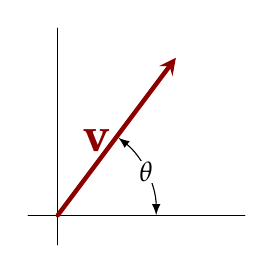
\begin{tikzpicture}[scale = 0.5, style={line cap = round}]
  % \filldraw [thick, white, draw=saitMaroon, drop shadow={opacity=0.25}] (-1, -1) rectangle (5,5);
  \draw (-0.75,0) -- (4.75,0);
  \draw (0, -0.75) -- (0, 4.75);
  \draw[ultra thick, saitMaroon, ->, >=stealth] (0, 0) -- (3, 4) node [xshift=-1cm, yshift=-1.05cm] {\LARGE ${\bm{\mathrm{ v }}}$};
  \only<2>{
    \draw[latex-latex] (2.5, 0) arc (0:52:2.5cm)  node[midway, fill=white, inner sep=0.1mm]{$\theta$};
  }
\end{tikzpicture}

		}
	}
	\uncover<2->{
		\hfill	
		\mini[0.6]{	
			\begin{statsbox}[left=0mm]{}
				\begin{itemize}
					\item $\theta$ indicates the direction of the line of action of the vector
								${\bm{\mathrm{ v }}}$  relative to some reference. \lb(I.e., the horizontal axis in this case.)
					
				\end{itemize}
			\end{statsbox}
		}
	}
\end{frame}

%%%%%%%%%%%%%%%%%%%%%%%%%%%%%%%%%%%%%%%%%%%%%%%%%%%%%%%%%%%%%%%%%%%%%%%%%%%%%%%%

\begin{frame}{Multiplication of a vector by a scalar}
	
	\cmini[0.8]{
		\begin{statsbox}[left=5mm, right=5mm]{}
			Multiplication of a vector by a scalar affects the magnitude and, if the scalar is negative, the sense of the direction of the vector.
			\parb	
			\centering
			% !TEX root = ../../statikz/statikz.tex

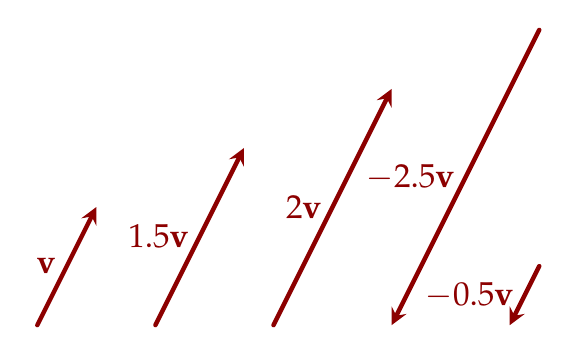
\begin{tikzpicture}[scale = 0.75, style={line cap = round}]

  % \filldraw [white, draw=saitMaroon, thick, drop shadow={opacity=0.25}] (-0.5, -1.5) rectangle (10,4.5);
  \draw[ultra thick, saitMaroon, ->, >=stealth] (0, -1) -- (1, 1) node [xshift=-0.375cm, yshift=-0.75cm, left] {\large ${\bm{\mathrm{ v }}}$};
  \draw[ultra thick, saitMaroon, ->, >=stealth] (2, -1) -- (3.5, 2) node [xshift=-0.5625cm, yshift=-1.125cm, left] {\large ${1.5 \bm{\mathrm{ v }}}$};
  \draw[ultra thick, saitMaroon, ->, >=stealth] (4, -1) -- (6, 3) node [xshift=-0.75cm, yshift=-1.5cm, left] {\large ${2 \bm{\mathrm{ v }}}$};
  \draw[ultra thick, saitMaroon, <-, >=stealth] (6, -1) -- (8.5, 4) node [xshift=-0.9375cm, yshift=-1.875cm, left] {\large ${-2.5 \bm{\mathrm{ v }}}$};
  \draw[ultra thick, saitMaroon, <-, >=stealth] (8, -1) -- (8.5, 0) node [xshift=-.1875cm, yshift=-.375cm, left] {\large ${-0.5 \bm{\mathrm{ v }}}$};

\end{tikzpicture}

		\end{statsbox}
	}
\end{frame}

%%%%%%%%%%%%%%%%%%%%%%%%%%%%%%%%%%%%%%%%%%%%%%%%%%%%%%%%%%%%%%%%%%%%%%%%%%%%%%%%

\begin{frame}{Addition of Vectors}
	% centered minipage with text raggedright
	%cmini[width]{content}
	\cmini[0.8]{

		\mini[0.5]{
			Consider two vectors, $\bm{\mathrm{ A }}$ and $\bm{\mathrm{ B }}$:
		}
		\hfill
		\mini[0.45]{
			\begin{statsbox}[top=0mm]{}
				\centering
				% !TEX root = ../../statikz/statikz.tex

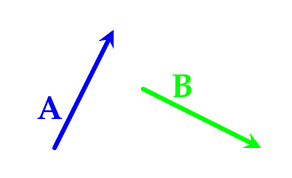
\begin{tikzpicture}[scale =0.75, style={line cap = round}]
  % \filldraw [white, draw=saitMaroon, thick, drop shadow={opacity=0.25}] (0.5, 0.5) rectangle (5,3.5);
  \draw[ultra thick, blue, ->, >=stealth] (1, 1) -- (2, 3) node [xshift=-0.5cm, yshift=-1cm, left] {\large ${\bm{\mathrm{ A }}} $};
  \draw[ultra thick, green, ->, >=stealth] (2.5, 2) -- (4.5, 1) node [xshift=-1cm, yshift=0.5cm, above] {\large ${\bm{\mathrm{ B }}}$};
\end{tikzpicture}

			\end{statsbox}			
		}
		\parm\pause
		\mini[0.5]{
			To add vectors  $\bm{\mathrm{ A }}$ and  $\bm{\mathrm{ B }}$, written $\bm{\mathrm{ A+B }}$, place the tail of $\bm{\mathrm{ B }}$ at the tip of~$\bm{\mathrm{ A }}$.
		}
		\hfill
		\mini[0.45]{
			\begin{statsbox}[top=0mm]{}
				\centering
				% !TEX root = ../../statikz/statikz.tex

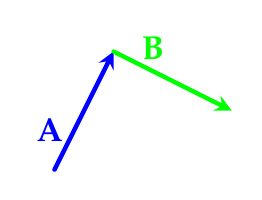
\begin{tikzpicture}[scale =0.75, style={line cap = round}]
  % \filldraw [white, draw=saitMaroon, thick, drop shadow={opacity=0.25}] (0.5, 0.5) rectangle (5,3.5);
  \draw[ultra thick, blue, ->, >=stealth] (1, 1) -- (2, 3) node [xshift=-0.5cm, yshift=-1cm, left] {\large ${\bm{\mathrm{ A }}}$};
  \draw[ultra thick, green, ->, >=stealth] (2, 3) -- (4, 2) node [xshift=-1cm, yshift=0.5cm, above] {\large ${\bm{\mathrm{ B }}}$};
\end{tikzpicture}

			\end{statsbox}			
		}
		\parm\pause
		\mini[0.5]{
			The sum, $\bm{ A+B}$, is obtained by drawing a vector ${\bm R}$ from the tail of $\bm{\mathrm{ A }}$ to the tip of $\bm{\mathrm{ B }}$.
			\[ \bm{\mathrm{A+B=R}} \]
		}
		\hfill
		\mini[0.45]{
			\begin{statsbox}[top=0mm]{}
				\centering
				% !TEX root = ../../statikz/statikz.tex

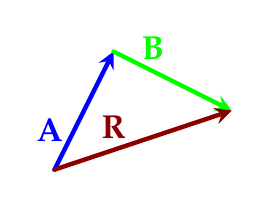
\begin{tikzpicture}[scale =0.75, style={line cap = round}]
  % \filldraw [white, draw=saitMaroon, thick, drop shadow={opacity=0.25}] (0.5, 0.5) rectangle (4.5,3.5);
  \draw[ultra thick, blue, ->, >=stealth] (1, 1) -- (2, 3) node [xshift=-0.5cm, yshift=-1cm, left] {\large ${\bm{\mathrm{ A }}}$};
  \draw[ultra thick, green, ->, >=stealth] (2, 3) -- (4, 2) node [xshift=-1cm, yshift=0.5cm, above] {\large ${\bm{\mathrm{ B }}}$};
  \draw[ultra thick, saitMaroon, ->, >=stealth] (1, 1) -- (4, 2) node [xshift=-1.5cm, yshift=-0.5cm, above] {\large ${\bm{\mathrm{ R }}}$};
\end{tikzpicture}

			\end{statsbox}			
		}
		\parm\pause
		\cmini[0.9]{
			{\bf Note that the sum of two vectors is itself a vector.}
		}

	}
\end{frame}

%%%%%%%%%%%%%%%%%%%%%%%%%%%%%%%%%%%%%%%%%%%%%%%%%%%%%%%%%%%%%%%%%%%%%%%%%%%%%%%%

\begin{frame}{Addition of Vectors :: It's commutative!}
	% centered minipage with text raggedright
	%cmini[width]{content}
	\cmini[0.6]{
		\mini[0.4]{
			\[ \bm{\mathrm{A+B=R}} \]
		}
		\hfill
		\mini[0.55]{
			\begin{statsbox}{}
				\centering
				% !TEX root = ../../statikz/statikz.tex

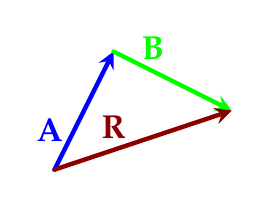
\begin{tikzpicture}[scale =0.75, style={line cap = round}]
  % \filldraw [white, draw=saitMaroon, thick, drop shadow={opacity=0.25}] (0.5, 0.5) rectangle (4.5,3.5);
  \draw[ultra thick, blue, ->, >=stealth] (1, 1) -- (2, 3) node [xshift=-0.5cm, yshift=-1cm, left] {\large ${\bm{\mathrm{ A }}}$};
  \draw[ultra thick, green, ->, >=stealth] (2, 3) -- (4, 2) node [xshift=-1cm, yshift=0.5cm, above] {\large ${\bm{\mathrm{ B }}}$};
  \draw[ultra thick, saitMaroon, ->, >=stealth] (1, 1) -- (4, 2) node [xshift=-1.5cm, yshift=-0.5cm, above] {\large ${\bm{\mathrm{ R }}}$};
\end{tikzpicture}

			\end{statsbox}			
		}
		\parm
		\mini[0.4]{
			\[ \bm{\mathrm{B+A=R}} \]
		}
		\hfill
		\mini[0.55]{
			\begin{statsbox}{}
				\centering
				% !TEX root = ../../statikz/statikz.tex

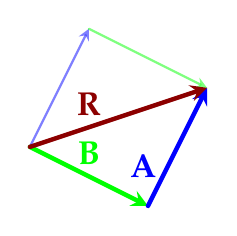
\begin{tikzpicture}[scale =0.75, style={line cap = round}]
  % \filldraw [white, draw=saitMaroon, thick, drop shadow={opacity=0.25}] (0.5, -0.5) rectangle (4.5,3.5);
  \draw[thick, blue, ->, >=stealth, opacity=0.5] (1, 1) -- (2, 3) ;
  \draw[thick, green, ->, >=stealth, opacity=0.5] (2, 3) -- (4, 2) ;

  \draw[ultra thick, green, ->, >=stealth] (1, 1) -- (3, 0) node [xshift=-0.75cm, yshift=0.375cm, above] {\large ${\bm{\mathrm{ B }}}$};
  \draw[ultra thick, blue, ->, >=stealth] (3, 0) -- (4, 2) node [xshift=-0.5cm, yshift=-1cm, left] {\large ${\bm{\mathrm{ A }}}$};

  \draw[ultra thick, saitMaroon, ->, >=stealth] (1, 1) -- (4, 2) node [xshift=-1.5cm, yshift=-0.5cm, above] {\large ${\bm{\mathrm{ R }}}$};
\end{tikzpicture}

			\end{statsbox}			
		}
		\parm\centering\pause

		\tcb[left=5mm, right=5mm, top=2mm, bottom=2mm]{%
			$\bm{\mathrm{A+B=B+A}}$
		}
	}
\end{frame}

%%%%%%%%%%%%%%%%%%%%%%%%%%%%%%%%%%%%%%%%%%%%%%%%%%%%%%%%%%%%%%%%%%%%%%%%%%%%%%%%

\begin{frame}{Addition of Vectors}

	% centered minipage with text raggedright
	%cmini[width]{content}
	\cmini[0.8]{
		\begin{myexam}{Displacement Vectors}{}
			\raggedright
			A displacement is a change in position. It has a magnitude (the distance moved) and a direction, so displacement is a vector quantity.\parm
			A truck drives due east on a straight road for 40 km, then drives north on a straight road for 30 km before stopping. \parb
			What is the resultant displacement of the truck?
		\end{myexam}
	}
	% \parb
	% \begin{center}
	% 	\footnotesize
	% 	\rotatebox[origin=c]{180}{
	% 		\textcolor{gray}{
	% 			($50\text{ km at }36.9^\circ \text{ North of East.}$)
	% 		}
	% 	}
	% \end{center}

\end{frame}

%%%%%%%%%%%%%%%%%%%%%%%%%%%%%%%%%%%%%%%%%%%%%%%%%%%%%%%%%%%%%%%%%%%%%%%%%%%%%%%

\begin{frame}{Addition of Vectors}
	\cmini[0.8]{
		\begin{myexam}{Velocity Vectors}{}
			\raggedright
			A plane flies NNW (i.e., $22.5\deg$ west of north) with a velocity of $275\text{ km/h}$. There is a wind blowing at $55\text{ km/h}$ from the NW (i.e., $45\deg$ west of north).
			\parb Determine the resultant velocity of the plane relative to the ground.
			\parb Determine the wind speed that would cause the plane to fly due north. What is the ground speed in this case?
		\end{myexam}
	}
	% \begin{center}
	% 	\footnotesize
	% 	\rotatebox[origin=c]{180}{
	% 		\textcolor{gray}{
	% 			($225\text{ km/h at} 17.1^\circ$ W of N, $149$ km/h wind speed and $149$ km/h ground speed)
	% 		}
	% 	}
	% \end{center}

\end{frame}

%%%%%%%%%%%%%%%%%%%%%%%%%%%%%%%%%%%%%%%%%%%%%%%%%%%%%%%%%%%%%%%%%%%%%%%%%%%%%%%%

\begin{frame}{The Parallelogram Law and the Triangle Law of Vector Addition}

	% centered minipage with text raggedright
	%cmini[width]{content}
	\cmini[0.9]{

		\mini[0.6]{
			{\bf The Parallelogram Law}:
			\begin{enumerate}
				\item  Draw the vectors with their tails at the same point.
				\item Form a parallelogram
				\item The diagonal of the parallelogram, starting from the tails of the two vectors, is the resultant.
			\end{enumerate}
		}
		\mini[0.35]{
			\begin{statsbox}{}
				\centering
				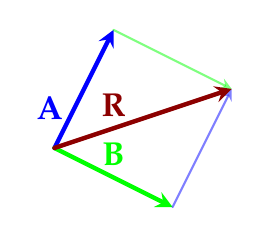
\begin{tikzpicture}[scale = 0.75, style={line cap = round}]
  % \filldraw [white, draw=saitMaroon, thick, drop shadow={opacity=0.25}] (0.5, -0.5) rectangle (4.5,3.5);
  \draw[ultra thick, blue, ->, >=stealth] (1, 1) -- (2, 3) node [xshift=-0.5cm, yshift=-1cm, left] {\large ${\bm{\mathrm{ A }}}$};
  \draw[thick, green, ->, >=stealth, opacity=0.5] (2, 3) -- (4, 2) ;
  \draw[ultra thick, green, ->, >=stealth] (1, 1) -- (3, 0) node [xshift=-0.75cm, yshift=0.375cm, above] {\large ${\bm{\mathrm{ B }}}$};
  \draw[thick, blue, ->, >=stealth, opacity=0.5] (3, 0) -- (4, 2);
  \draw[ultra thick, saitMaroon, ->, >=stealth] (1, 1) -- (4, 2) node [xshift=-1.5cm, yshift=-0.5cm, above] {\large ${\bm{\mathrm{ R }}}$};
\end{tikzpicture}

			\end{statsbox}
			
		}
		\par\vspace{0.75cm}\pause
		\mini[0.6]{
			{\bf The Triangle Law}:
			\begin{enumerate}
				\item This is what we have been doing
				\item To do the calculations on the parallelogram above, we end up working with the triangle(s) anyway
				\item {\bf Use the triangle law}.
			\end{enumerate}
		}
		\hfill
		\mini[0.35]{
			\begin{statsbox}{}
				\centering
				% !TEX root = ../../statikz/statikz.tex

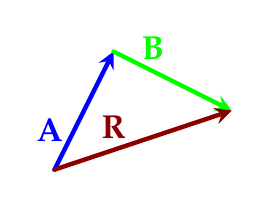
\begin{tikzpicture}[scale =0.75, style={line cap = round}]
  % \filldraw [white, draw=saitMaroon, thick, drop shadow={opacity=0.25}] (0.5, 0.5) rectangle (4.5,3.5);
  \draw[ultra thick, blue, ->, >=stealth] (1, 1) -- (2, 3) node [xshift=-0.5cm, yshift=-1cm, left] {\large ${\bm{\mathrm{ A }}}$};
  \draw[ultra thick, green, ->, >=stealth] (2, 3) -- (4, 2) node [xshift=-1cm, yshift=0.5cm, above] {\large ${\bm{\mathrm{ B }}}$};
  \draw[ultra thick, saitMaroon, ->, >=stealth] (1, 1) -- (4, 2) node [xshift=-1.5cm, yshift=-0.5cm, above] {\large ${\bm{\mathrm{ R }}}$};
\end{tikzpicture}

			\end{statsbox}
		}
		% \parb
		% You can check out an interactive visualization of the parallelogram law and the triangle law \href{http://eduk8r.org/jsSims/statics/vectorAddition/}{\bf here}.
	}
\end{frame}

%%%%%%%%%%%%%%%%%%%%%%%%%%%%%%%%%%%%%%%%%%%%%%%%%%%%%%%%%%%%%%%%%%%%%%%%%%%%%%%%

\begin{frame}{Subtraction of Vectors}
	
		\tb[0.5\columnwidth]{0.5in}{0.875in}{	
			\begin{itemize}
				\item Consider two vectors, $\bm{\mathrm{ A }}$ and $\bm{\mathrm{ B }}$:
			\end{itemize}	
			
		}
		\tb[0.4\columnwidth]{2.625in}{0.625in}{
			\begin{statsbox}[top=0mm]{}
				\centering
				% !TEX root = ../../statikz/statikz.tex

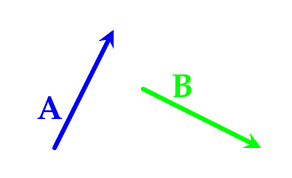
\begin{tikzpicture}[scale =0.75, style={line cap = round}]
  % \filldraw [white, draw=saitMaroon, thick, drop shadow={opacity=0.25}] (0.5, 0.5) rectangle (5,3.5);
  \draw[ultra thick, blue, ->, >=stealth] (1, 1) -- (2, 3) node [xshift=-0.5cm, yshift=-1cm, left] {\large ${\bm{\mathrm{ A }}}$};
  \draw[ultra thick, green, ->, >=stealth] (2.5, 2) -- (4.5, 1) node [xshift=-1cm, yshift=0.5cm, above] {\large ${\bm{\mathrm{ B }}}$};
\end{tikzpicture}

			\end{statsbox}			
		}
		
		\tb[0.45\columnwidth]{0.5in}{1.625in}{
			\uncover<2->{
				\raggedright
				\begin{itemize}
					\item Now consider $\bm{\bm\mathrm{ -B }}$, which is obtained by reversing the sense of $\bm{\mathrm{ B }}$.
				\end{itemize}	
			}		
		}
		\tb[0.4\columnwidth]{2.625in}{1.4625in}{
			\uncover<2->{
				\begin{statsbox}[top=0mm]{}
					\centering
					% !TEX root = ../../statikz/statikz.tex

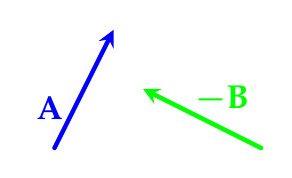
\begin{tikzpicture}[scale =0.75, style={line cap = round}]
  % \filldraw [white, draw=saitMaroon, thick, drop shadow={opacity=0.25}] (0.5, 0.5) rectangle (5,3.5);
  \draw[ultra thick, blue, ->, >=stealth] (1, 1) -- (2, 3) node [xshift=-0.5cm, yshift=-1cm, left] {\large $\bm{\mathrm{ A }}$};
  \draw[ultra thick, green, <-, >=stealth] (2.5, 2) -- (4.5, 1) node [xshift=-0.5cm, yshift=0.3cm, above] {\large $\bm{\mathrm{ -B }}$};
\end{tikzpicture}

				\end{statsbox}
			}
		}
		\tb[0.45\columnwidth]{0.5in}{2.5in}{
			\uncover<3->{
				\begin{itemize}
					\item Then, add  $\bm{\mathrm{ A }}$ to $\bm{\mathrm{ -B }}$:\vspace{-1.5em}
					
						\begin{align*}
							\bm{A-B} & = \bm{\mathrm{ A+(-B) }} \\
											& =\bm{\mathrm{ R }}
						\end{align*}
				\end{itemize}
			}
		}
	
		\tb[0.4\columnwidth]{2.625in}{2.375in}{
			\uncover<3->{
				\begin{statsbox}[top=0mm]{}
					\centering
					

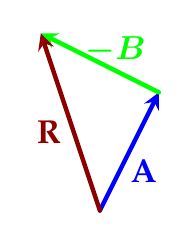
\begin{tikzpicture}[scale =0.75, style={line cap = round}] 
  \draw[ultra thick, blue, ->, >=stealth] (2.5, 1) -- +(1, 2) node [xshift=-0.5cm, yshift=-1cm, right] {\large ${\bm{\mathrm{ A }}}$};
  \draw[ultra thick, green, ->, >=stealth] (3.5, 3) -- +(-2, 1) node [xshift=0.95cm, yshift=0.1cm, below] {\large $\bm{ -B }$};
  \draw[ultra thick, saitMaroon, ->, >=stealth] (2.5, 1) -- +(-1, 3) node [xshift=.4cm, yshift=-1.25cm, left] {\large ${\bm{\mathrm{ R }}}$};
\end{tikzpicture}

				\end{statsbox}
			}
		}
	
\end{frame}

%%%%%%%%%%%%%%%%%%%%%%%%%%%%%%%%%%%%%%%%%%%%%%%%%%%%%%%%%%%%%%%%%%%%%%%%%%%%%%%%

\begin{frame}{Addition of Several Vectors}
	% textblock*
	\tb[1.75in]{0.5in}{1in}{
		Consider the sum of vectors $\bm{\mathrm{ A }}$, $\bm{\mathrm{ B }}$, $\bm{\mathrm{ C }}$, $\bm{\mathrm{ D }}$, $\bm{\mathrm{ E }}$ and $\bm{\mathrm{ F }}$:
	}
	\tb[2in]{2.5in}{0.58in}{
		\begin{statsbox}[top=0mm]{}
			\centering
			% !TEX root = ../../statikz/statikz.tex

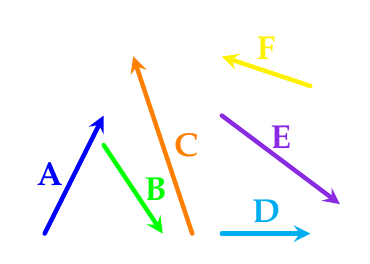
\begin{tikzpicture}[scale =0.75, style={line cap = round}]
  % \filldraw [white, draw=saitMaroon, thick, drop shadow={opacity=0.25}] (0.5, 0.5) rectangle (6.5,4.5);
  \draw[ultra thick, blue, ->, >=stealth] (1, 1) -- node[left] {\large ${\bm{\mathrm{ A }}}$} ++(1, 2);
  \draw[ultra thick, green, ->, >=stealth] (2, 2.5) -- node[right]{\large ${\bm{\mathrm{ B }}}$} ++ (1, -1.5);
  \draw[ultra thick, orange, ->, >=stealth] (3.5, 1) -- node[right]{\large ${\bm{\mathrm{ C }}}$} ++ (-1, 3);
  \draw[ultra thick, cyan, ->, >=stealth] (4, 1) -- node[above]{\large ${\bm{\mathrm{ D }}}$} ++ (1.5, 0);
  \draw[ultra thick, BlueViolet, ->, >=stealth] (4, 3) -- node[above]{\large ${\bm{\mathrm{ E }}}$} ++ (2, -1.5);
  \draw[ultra thick, yellow, ->, >=stealth] (5.5, 3.5) -- node[above]{\large ${\bm{\mathrm{ F }}}$} ++ (-1.5, .5);
\end{tikzpicture}

		\end{statsbox}
	}
	\uncover<2->{
		\tb[1.75in]{0.5in}{1.925in}{
			\begin{itemize}
				\item<2-> Place all the vectors nose to tail.
				\item<3-> Analyze the triangles. There are five sets of triangle calculations to do.
				\item<8-> {\bf This is too much work!} We will find a more efficient way soon :)
			\end{itemize}
		}
			\hfill
			\tb[2in]{2.5in}{1.875in}{
				\centering
				\uncover<2->{
					\begin{statsbox}{}
						\centering
						% !TEX root = ../../statikz/statikz.tex

\begin{tikzpicture}[scale =0.75]
  % \filldraw [white, draw=saitMaroon, thick, drop shadow={opacity=0.25}] (0.5, 0.5) rectangle (6.5,5);
  % A and B
  \only<2>{
    \draw[line width=.4mm, green, ->, >=stealth] (2, 3) -- node[left]{\large ${\bm{\mathrm{ B }}}$} ++ (1, -1.5);
    \draw[line width=.4mm, blue, ->, >=stealth] (1, 1) -- node[left] {\large ${\bm{\mathrm{ A }}}$} ++(1, 2);
  }
  \only<3>{
    \draw[line width=.4mm, green, ->, >=stealth, opacity=0.4] (2, 3) -- node[left]{\large ${\bm{\mathrm{ B }}}$} ++ (1, -1.5);
    \draw[line width=.4mm, blue, ->, >=stealth, opacity=0.4] (1, 1) -- node[left] {\large ${\bm{\mathrm{ A }}}$} ++(1, 2);
  }
  \only<4->{
    \draw[line width=.4mm, green, ->, >=stealth, opacity=0.1] (2, 3) -- node[left]{\large ${\bm{\mathrm{ B }}}$} ++ (1, -1.5);
    \draw[line width=.4mm, blue, ->, >=stealth, opacity=0.1] (1, 1) -- node[left] {\large ${\bm{\mathrm{ A }}}$} ++(1, 2);
  }
  % C and D
  \only<2-3>{
    \draw[line width=.4mm, cyan, ->, >=stealth] (2,4.5) -- node[below]{\large ${\bm{\mathrm{ D }}}$} ++ (1.5, 0);
    \draw[line width=.4mm, orange, ->, >=stealth] (3, 1.5) -- node[right]{\large ${\bm{\mathrm{ C }}}$} ++ (-1, 3);
  }
  \only<4>{
    \draw[line width=.4mm, cyan, ->, >=stealth, opacity=0.4] (2,4.5) -- node[below]{\large ${\bm{\mathrm{ D }}}$} ++ (1.5, 0);
    \draw[line width=.4mm, orange, ->, >=stealth, opacity=0.4] (3, 1.5) -- node[right]{\large ${\bm{\mathrm{ C }}}$} ++ (-1, 3);
  }
  \only<5->{
    \draw[line width=.4mm, cyan, ->, >=stealth, opacity=0.1] (2,4.5) -- node[below]{\large ${\bm{\mathrm{ D }}}$} ++ (1.5, 0);
    \draw[line width=.4mm, orange, ->, >=stealth, opacity=0.1] (3, 1.5) -- node[right]{\large ${\bm{\mathrm{ C }}}$} ++ (-1, 3);
  }
  % E and F
  \only<2-4>{
    \draw[line width=.4mm, yellow, ->, >=stealth] (5.5, 3) -- node[below]{\large ${\bm{\mathrm{ F }}}$} ++ (-1.5, .5);
    \draw[line width=.4mm, BlueViolet, ->, >=stealth] (3.5, 4.5) -- node[above]{\large ${\bm{\mathrm{ E }}}$} ++ (2, -1.5);
  }
  \only<5>{
    \draw[line width=.4mm, yellow, ->, >=stealth, opacity=0.4] (5.5, 3) -- node[below]{\large ${\bm{\mathrm{ F }}}$} ++ (-1.5, .5);
    \draw[line width=.4mm, BlueViolet, ->, >=stealth, opacity=0.4] (3.5, 4.5) -- node[above]{\large ${\bm{\mathrm{ E }}}$} ++ (2, -1.5);
  }
  \only<6->{
    \draw[line width=.4mm, yellow, ->, >=stealth, opacity=0.1] (5.5, 3) -- node[below]{\large ${\bm{\mathrm{ F }}}$} ++ (-1.5, .5);
    \draw[line width=.4mm, BlueViolet, ->, >=stealth, opacity=0.1] (3.5, 4.5) -- node[above]{\large ${\bm{\mathrm{ E }}}$} ++ (2, -1.5);
  }
  % R's
  \only<6>{
    \draw[line width=.6mm, saitMaroon, ->, >=stealth] (1, 1) -- node[right] {\large $\bm{\mathrm{ R_4 }}$ } ++(2.5, 3.5);
  }
  % \only<7->{
  % 	\draw[line width=.6mm, saitMaroon, ->, >=stealth] (1, 1) -- node[right] {\large ${\bm R_4 }$} ++(2.5, 3.5);
  % }
  \only<3-5>{
    \draw[line width=.5mm, saitRed, ->, >=stealth] (1, 1) -- node[below] {\large $\bm{\mathrm{ R_1 }}$} ++(2, 0.5);
  }
  \only<4-5>{
    \draw[line width=.5mm, saitRed, ->, >=stealth] (3, 1.5) -- node[right] {\large $\bm{\mathrm{ R_2 }}$} ++(0.5, 3);
  }
  \only<6>{
    \draw[line width=.5mm, saitRed, ->, >=stealth, opacity=0.4] (1, 1) -- node[below] {\large $\bm{\mathrm{ R_1 }}$} ++(2, 0.5);
    \draw[line width=.5mm, saitRed, ->, >=stealth, opacity=0.4] (3, 1.5) -- node[right] {\large $\bm{\mathrm{ R_2 }}$} ++(0.5, 3);
  }
  \only<7->{
    \draw[line width=.6mm, saitMaroon!70!black, ->, >=stealth] (1, 1) -- node[below right] {\large $\bm{\mathrm{ R_5 }}$} ++(3, 2.5);
    \draw[line width=.6mm, saitMaroon, ->, >=stealth, opacity=0.1] (1, 1) -- node[right] {\large $\bm{\mathrm{ R_4 }}$} ++(2.5, 3.5);
    \draw[line width=.5mm, saitRed, ->, >=stealth, opacity=0.1] (3.5, 4.5) -- node[right] {\large $\bm{\mathrm{ R_3 }}$} ++(0.5, -1);
    \draw[line width=.5mm, saitRed, ->, >=stealth, opacity=0.1] (1, 1) -- node[below] {\large ${\bm R_1 }$} ++(2, 0.5);
    \draw[line width=.5mm, saitRed, ->, >=stealth, opacity=0.1] (3, 1.5) -- node[right] {\large $\bm{\mathrm{ R_2 }}$} ++(0.5, 3);
  }
  \only<5-6>{
    \draw[line width=.5mm, saitRed, ->, >=stealth] (3.5, 4.5) -- node[right] {\large $\bm{\mathrm{ R_3 }}$} ++(0.5, -1);
  }
\end{tikzpicture}

					\end{statsbox}
					
				}
			}
		}
	
\end{frame}

%%%%%%%%%%%%%%%%%%%%%%%%%%%%%%%%%%%%%%%%%%%%%%%%%%%%%%%%%%%%%%%%%%%%%%%%%%%%%%%%

\begin{frame}{Vector Addition of Forces}
	% centered minipage with text raggedright
	%cmini[width]{content}
	\cmini[0.8]{
		\begin{itemize}
			\item {\bf Force} is a vector quantity. It has a magnitude and a direction.\pars
			\item Consider your weight. It is a force; it has a magnitude (newtons or pounds). It has a direction (along a line of action that passes between you and the centre of the earth). And it has a sense: down, towards the centre of the earth. If you step off a diving board, you will accelerate downwards in a predictable fashion. \pars
			\item We have seen that we can add vectors together so we can do the same for forces.\pars
			\item Multiple forces acting on an object through a point have a \textcolor{structure}{\bf resultant} force (the net force,  which is the combined result of the summing together of the multiple forces).\pars
			\item The forces which, when combined, sum to this resultant are known as \textcolor{structure}{\bf component} forces.
		\end{itemize}
	}
\end{frame}

%%%%%%%%%%%%%%%%%%%%%%%%%%%%%%%%%%%%%%%%%%%%%%%%%%%%%%%%%%%%%%%%%%%%%%%%%%%%%%%%

\begin{frame}{Resultants and Components}

	
		\mini[0.44]{
			\begin{itemize}
				\item Consider forces $\bm{\mathrm{ A }}$ and $\bm{\mathrm{ B }}$ acting at point $0$, as shown.\parm
				\item<2-> The \textcolor{statsMaroon}{\bf resultant} force, $\bm{\mathrm{ R }}$, of forces $\bm{\mathrm{ A }}$ and $\bm{\mathrm{ B }}$ is the \textcolor{statsMaroon}{\bf vector sum} of $\bm{\mathrm{ A }}$ and $\bm{\mathrm{ B }}$. \parm
				\item<3-> $\bm{\mathrm{ A }}$ and $\bm{\mathrm{ B }}$ are \textcolor{statsMaroon}{\bf component} forces of $\bm{\mathrm{ R }}$. \parm
				\item<4-> $\bm{\mathrm{ C }}$ and $\bm{\mathrm{ D }}$ are also \textcolor{statsMaroon}{\bf component} forces of  $\bm{\mathrm{ R }}$. \parm
				\item<5->\ldots as are $\bm{\mathrm{ E}}$ and $\bm{\mathrm{ F }}$ \parm
				\item<6->There are infinitely many possible component forces for each force  $\bm{\mathrm{ R }}$
			\end{itemize}
		}
		\hfill
		\mini[0.45]{
			\begin{statsbox}[top=0mm, right=0mm, bottom=0mm, left=0mm]{}
				\centering
				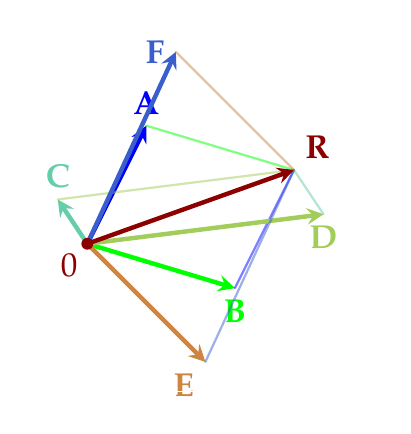
\begin{tikzpicture}[scale = 0.75, style={line cap = round}]
  \coordinate (O) at (0,0);
  \coordinate (A) at (1,2);
  \coordinate (B) at (2.5,-0.75);
  \coordinate (R) at (3.5,1.25);
  \coordinate (C) at (-0.5,0.75);
  \coordinate (D) at (4,0.5);
  \coordinate (E) at (2,-2);
  \coordinate (F) at (1.5,3.25);

  \uncover<1-3>{
  \draw[ultra thick, blue, ->, >=stealth] (O) -- (A) node [above] {\large ${\bm{\mathrm{ A }}}$};
  \draw[ultra thick, green, ->, >=stealth] (O) -- (B) node [below] {\large ${\bm{\mathrm{ B }}}$};
  }
  \uncover<2-3>{
    \draw[thick, blue, opacity=0.5] (B) -- (R) ;
    \draw[thick, green, opacity=0.5] (A) -- (R) ;
  }
 
  
  \uncover<4>{
    \draw[ultra thick, Aquamarine3, ->, >=stealth] (O) -- (C) node [above] {\large ${\bm{\mathrm{ C }}}$};
    \draw[ultra thick, DarkOliveGreen3, ->, >=stealth] (O) -- (D) node [below] {\large ${\bm{\mathrm{ D }}}$};
    \draw[thick, DarkOliveGreen3, opacity=0.5] (C) -- (R) ;
    \draw[thick, Aquamarine3, opacity=0.5] (D) -- (R) ;
  }
  \uncover<5->{
    \draw[ultra thick, Tan3, ->, >=stealth] (O) -- (E) node [below left] {\large ${\bm{\mathrm{ E }}}$};
    \draw[ultra thick, RoyalBlue3, ->, >=stealth] (O) -- (F) node [left] {\large ${\bm{\mathrm{ F }}}$};
    \draw[thick, RoyalBlue3, opacity=0.5] (E) -- (R) ;
    \draw[thick, Tan3, opacity=0.5] (F) -- (R) ;
  }
  
  \uncover<2->{
  \draw[ultra thick, statsMaroon, ->, >=stealth] (O) -- (R) node [above right] {\large ${\bm{\mathrm{ R }}}$};
  }
  \fill[statsMaroon] (O) circle (1mm) node[below left] {\large $0$};
  \draw[white] (-1,3.65) rectangle (5,-2.5);
\end{tikzpicture}

			\end{statsbox}
		}
	

\end{frame}

%%%%%%%%%%%%%%%%%%%%%%%%%%%%%%%%%%%%%%%%%%%%%%%%%%%%%%%%%%%%%%%%%%%%%%%%%%%%%%%%


\begin{frame}{Finding Resultants and Components}
	\begin{itemize}
		\item In each of the examples just given, there were only two components but there can be many components for each resultant.\parm

	\end{itemize}

	\parm
	% left-aligned minipage with text raggedright
	%mini[width]{content}
	\mini[0.45]{
		\begin{itemize}
			\item<2-> In this case, $\bm{\mathrm{ R }}$ is the resultant of $6$ component forces: $\bm{\mathrm{ A }}$, $\bm{\mathrm{ B }}$, $\bm{\mathrm{ C }}$, $\bm{\mathrm{ D }}$, $\bm{\mathrm{ E }}$ and $\bm{\mathrm{ F }}$\parb
			\item<3-> In this course, for each force $\bm{R}$ we shall generally need only two components.
		\end{itemize}
	}
	\hfill
	\mini[0.45]{
		\begin{statsbox}{}
			\centering
			% !TEX root = ../../statikz/statikz.tex

\begin{tikzpicture}[scale =0.75]
  \only<1>{
    \draw[very thick, Goldenrod3, -latex] (5.5, 3) -- +(-1.5, .5) node[below right, yshift=-0.1cm]{ ${\bm{\mathrm{ F }}}$}; 
    \draw[very thick, BlueViolet, ->, -latex] (3.5, 4.5) -- +(2, -1.5) node[above]{ ${\bm{\mathrm{ E }}}$};
    \draw[very thick, cyan, -latex] (2,4.5) -- + (1.5, 0) node[above]{ ${\bm{\mathrm{ D }}}$} ;
    \draw[very thick,Orange1, -latex] (3, 1.5) -- ++ (-1, 3) node[left]{ ${\bm{\mathrm{ C }}}$} ;
    \draw[very thick, green, -latex] (2, 3) -- ++ (1, -1.5)node[left,xshift=-0.5mm]{ ${\bm{\mathrm{ B }}}$} ;
    \draw[very thick, blue, -latex] (1, 1) -- ++(1, 2)node[left,xshift=-0.5mm] { ${\bm{\mathrm{ A }}}$} ;
  }
  \only<2->{
    \draw[very thick, Goldenrod3, -latex, opacity=0.4] (5.5, 3) -- +(-1.5, .5) node[below right, yshift=-0.1cm]{ ${\bm{\mathrm{ F }}}$}; 
    \draw[very thick, BlueViolet, ->, -latex, opacity=0.4] (3.5, 4.5) -- +(2, -1.5) node[above]{ ${\bm{\mathrm{ E }}}$};
    \draw[very thick, cyan, -latex, opacity=0.4] (2,4.5) -- + (1.5, 0) node[above]{ ${\bm{\mathrm{ D }}}$} ;
    \draw[very thick,Orange1, -latex, opacity=0.4] (3, 1.5) -- ++ (-1, 3) node[left]{ ${\bm{\mathrm{ C }}}$} ;
    \draw[very thick, green, -latex, opacity=0.4] (2, 3) -- ++ (1, -1.5)node[left,xshift=-0.5mm]{ ${\bm{\mathrm{ B }}}$};
    \draw[very thick, blue, -latex, opacity=0.4] (1, 1) -- ++(1, 2)node[left,xshift=-0.5mm] { ${\bm{\mathrm{ A }}}$};
    \draw[ultra thick, statsMaroon, -latex] (1, 1) -- (4, 3.5)node[left,xshift=-3mm, yshift=-1.5mm] { ${\bm{\mathrm{ R }}}$};


  }
\end{tikzpicture}

		\end{statsbox}
		
	}
\end{frame}



%%%%%%%%%%%%%%%%%%%%%%%%%%%%%%%%%%%%%%%%%%%%%%%%%%%%%%%%%%%%%%%%%%%%%%%%%%%%%%%%

\begin{frame}{Resultant Forces}
	
	\begin{myexam}{}{}

		Determine the magnitude and the direction (measured clockwise from the the positive $x$-axis) of the resultant of the two forces. \parm\centering
		{\bf Note}: One kilonewton is one thousand newtons, i.e., $1\,\mathsf{kN} = 1000\,\mathsf{N}$
		\parb

		\begin{center}
			\def\scale{0.9}
			\begin{tikzpicture}[scale=\scale, line cap=round,
			postaction=decorate,
  		decoration = {markings, mark = between positions 0
  		and 1 step 16pt with 
				{
					\begin{scope}[scale=0.8]
						\draw[statsMaroon, very thick]  (0, -3pt)--++(3pt, 0)arc(-90:90:3pt)--++(-6pt,0)arc(90:270:3pt)--cycle;
						\draw[statsMaroon,ultra thick] (-16pt,0) -- (-4pt,0); 
					\end{scope}
				}
			}
		]

	\coordinate (D) at (-3,1);
	\coordinate (E) at (3, 2);
	\coordinate (C) at (0, 0);

	\fill[mucus!50] (D) rectangle (E);
	\draw[thin, black] (D) -- ($(E)-(0,1) $);
	\EyeConnection[180]{C}{mucus!50}{black}{1}{0.5};

	\draw[latex-latex] ($ (C)+(180:2.12)$) arc (180:225:2.12) node[fill=white, midway, inner sep=0.25mm] {$ 45\deg $};
	\draw[latex-latex] ($ (C)+(0:2.12)$) arc (0:-30:2.12) node[fill=white, midway, inner sep=0.25mm] {$ 30\deg $};


	\path[postaction={decorate}] ($ (C)+(-30:0.55) $) -- +(-30:2);
	\path[postaction={decorate}] ($ (C)+(225:0.55) $) -- +(225:2);
	\draw[line width=0.875mm, -latex, statsDeepBlue] ($ (C)+(-30:1.25) $) -- +(-30:2) node[black, right]{\(2.50\,\text{ kN}\)};
	\draw[line width=0.875mm, -latex, statsDeepBlue] ($ (C)+(225:1.25) $) -- +(225:2) node[black, left]{\(3.75\,\text{ kN}\)};

	\draw[thin] ($(C)+(-0.5,0) $) -- +(-2.25,0);
	\draw[thin] ($(C)+(0.5,0) $) -- +(2.25,0) node[right] {$x$};



	


\end{tikzpicture}

			% \footnotesize
			% \rotatebox[origin=c]{180}{
			% 	\textcolor{gray}{
			% 		($3.93$ kN at $97.1^\circ$ measured clockwise from the positive $x$ axis)
			% 	}
			% }
		\end{center}
	\end{myexam}

\end{frame}

%%%%%%%%%%%%%%%%%%%%%%%%%%%%%%%%%%%%%%%%%%%%%%%%%%%%%%%%%%%%%%%%%%%%%%%%%%%%%%%%

% \begin{frame}
% 	\begin{tikzpicture}[line cap = round,
% 			postaction=decorate,
%   		decoration = {markings, mark = between positions 0
%   		and 1 step 16pt with 
% 			{
% 				\draw[statsMaroon, ultra thick]  (0, -3pt)--++(3pt, 0)arc(-90:90:3pt)--++(-6pt,0)arc(90:270:3pt)--cycle;
%         \draw[red,ultra thick] (-13pt,0) -- (-3pt,0); 
% 			}
% 			}
% 			]
%       \path[postaction={decorate}](0,0) arc(180:0:1) arc(-180:0:1);
%       \path[postaction={decorate}](5,0) -- +(4,-2);
			
% 	\end{tikzpicture}
	
	

% \end{frame}

%%%%%%%%%%%%%%%%%%%%%%%%%%%%%%%%%%%%%%%%%%%%%%%%%%%%%%%%%%%%%%%%%%%%%%%%%%%%%%%%

\begin{frame}{Resultant Forces}

	\begin{myexer}{}{}
		\def\scale{0.8}
		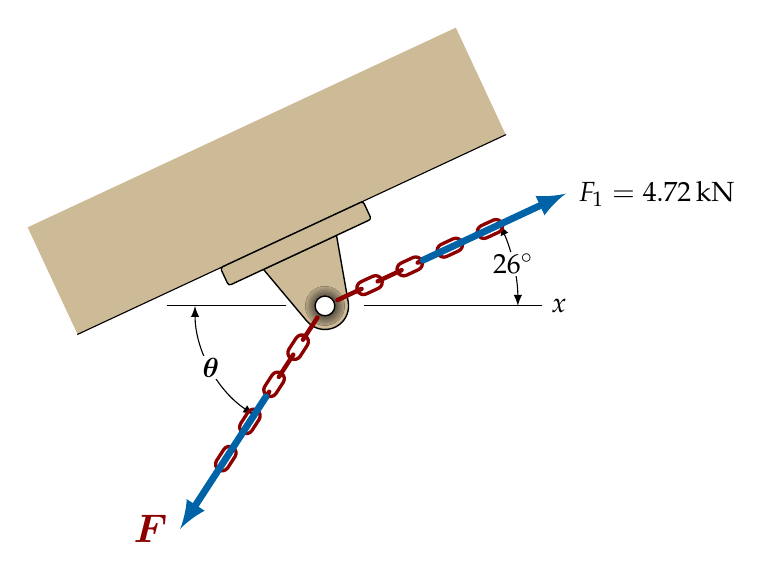
\begin{tikzpicture}[scale=\scale, line cap=round,
			postaction=decorate,
  		decoration = {markings, mark = between positions 0
  		and 1 step 16pt with 
				{
					\begin{scope}[scale=0.8]
						\draw[statsMaroon, very thick]  (0, -3pt)--++(3pt, 0)arc(-90:90:3pt)--++(-6pt,0)arc(90:270:3pt)--cycle;
						\draw[statsMaroon,ultra thick] (-16pt,0) -- (-4pt,0); 
					\end{scope}
				}
			}
		]

	\coordinate (D) at (-3,1);
	\coordinate (E) at (3, 2.5);
	\coordinate (C) at (0, 0);

\begin{scope}[rotate=25]
	\fill[Wheat3] (-3,1) rectangle (3,2.5);
	\draw[thin, black] (-3,1) -- ($(3,2.5)-(0,1.5)$);
	\EyeConnection[180]{C}{Wheat3}{black}{1}{0.5}
\end{scope}

	\draw[latex-latex] ($(C)+(180:1.65)$) arc (180:237:1.65) node[fill=white, midway, inner sep=0.25mm] {$\bm \theta$};
	\draw[latex-latex] ($(C)+(0:2.45)$) arc (0:25:2.45) node[fill=white, midway, inner sep=0.25mm] {$ 26^\circ $};


	\path[postaction={decorate}] ($(C)+(25:0.625)$) -- +(25:2);
	\path[postaction={decorate}] ($(C)+(237:0.625)$) -- +(237:2);
	\draw[line width=0.875mm, -latex, statsDeepBlue] ($(C)+(25:1.375)$) -- +(25:2) node[black, right]{$F_1=4.72\,\mathrm{kN}$};
	\draw[line width=0.875mm, -latex, statsDeepBlue] ($(C)+(237:1.375)$) -- +(237:2) node[statsMaroon, left]{\Large $\bm F $};

	\draw[thin] ($(C)+(-0.5,0)$) -- +(-1.5,0);
	\draw[thin] ($(C)+(0.5,0)$) -- +(2.25,0) node[right] {$x$};




\end{tikzpicture}

		\parb

		% \begin{center}
		% 	\footnotesize
		% 	\rotatebox[origin=c]{180}{
		% 		\textcolor{gray}{
		% 			($F = 4.32$ kN, $\theta = 66.3^\circ$)
		% 		}
		% 	}
		% \end{center}
	\end{myexer}

	\begin{textblock*}{0.5\textwidth}(5.5cm, 5.75cm)
		The resultant of the forces $F$ and $F_1$ is $3.14$ kN at $37^\circ$ clockwise from the positive $x$ axis.\parm
		Determine $F$ and $\theta$.

	\end{textblock*}

\end{frame}
%%%%%%%%%%%%%%%%%%%%%%%%%%%%%%%%%%%%%%%%%%%%%%%%%%%%%%%%%%%%%%%%%%%%%%%%%%%%%%%%


\begin{frame}{Mass, Force and Weight}
	\cmini{
		\begin{itemize}
			\item From Newton's Second Law of Motion, $\bm{F=ma}$ \lb(force = mass x acceleration)\parb
			\item The weight of an object is a force. It is the gravitational attractive force between the object and the earth.\parb
			\item If we denote the acceleration due to gravity by $\bm g$ ($g=9.81\mathsf{\;m/s^2}=32.2\mathsf{\;ft/s^2} $) and denote the mass of the object by $\bm m$, then the weight of the object, $\bm W$, is given by:
		\end{itemize}
		\parb
		\centering
		\begin{statsbox}[width=3cm, top=1mm]{}
			\[ W=mg \]
		\end{statsbox}
	}
\end{frame}

%%%%%%%%%%%%%%%%%%%%%%%%%%%%%%%%%%%%%%%%%%%%%%%%%%%%%%%%%%%%%%%%%%%%%%%%%%%%%%%%
\begin{frame}{Metric (SI) Units of Measurement}
	\cmini{
		\begin{itemize}
			\item There are four basic quantities involved in $F=ma$: force, mass, distance and time. \parb
			\item According to Newton, a net force of one newton ({\bfseries N}) causes a mass of one kilogram ({\bfseries kg}) to accelerate by\lb 1 metre/sec/sec ({\bfseries m/s}$\bm{^2}$).\parb
			\item A rock dropped from a bridge is subject to a gravitational attractive force and will have an acceleration of $9.81\mathsf{\;m/s^2}$. If the rock has a mass of $2.75\text{ kg}$, this force is given by:
			      \begin{align*}
			      	F & = ma                                        \\
			      	  & = 2.75\text{ kg}\times 9.81\mathsf{\;m/s^2} \\
			      	  & = 27.0\text{ N}
			      \end{align*}
			      This force $F$ is the weight, $W$, of the rock. So, $W=mg$
		\end{itemize}
	}
\end{frame}

%%%%%%%%%%%%%%%%%%%%%%%%%%%%%%%%%%%%%%%%%%%%%%%%%%%%%%%%%%%%%%%%%%%%%%%%%%%%%%%%
\begin{frame}{Metric (or SI) Units of Measurement}
	\cmini{
		To summarize:
		\begin{enumerate}
			\item $	1 \mathsf{\,N} = 1\mathsf{\,kg} \times 1\mathsf{\,m/s^2} = 1 \mathsf{\,kg\cdot m/s^2}$\parb
			\item To calculate the weight of an object from its mass, multiply the mass in kg by $g=9.81\,\mathsf{m/s^2}$. The weight is in newtons.\parb
			\item To calculate the mass of an object from its weight, divide the weight in newtons by
			      $g=9.81\,\mathsf{m/s^2}$. The mass is in kilograms.
		\end{enumerate}

	}
\end{frame}


%%%%%%%%%%%%%%%%%%%%%%%%%%%%%%%%%%%%%%%%%%%%%%%%%%%%%%%%%%%%%%%%%%%%%%%%%%%%%%%%

\begin{frame}{US Customary (or Imperial) Units of Measurement}
	\cmini{
		\begin{itemize}
			\item Acceleration due to gravity in feet and seconds is $$g=32.2\,\mathsf{ft/s^2}$$
			\item The unit for force is the pound, or {\bf lb}. \lb(It may also be described as pound-force, or {\bf lbf}.)\parb
			\item The unit for mass is the {\bfseries slug}.\parb
			\item	 $	1 \mathsf{lb} = 1\mathsf{\,slug} \times 1\mathsf{\,ft/s^2} \Rightarrow 1 \mathsf{\,slug}$ has the units $\frac{\mathsf{lb\cdot sec}}{\mathsf{ft^2}}$\parb
			\item To calculate the mass of an object from its weight, divide the weight in pounds by
			      $g=32.2\,\mathsf{ft/s^2}$. The mass is in slugs.\parb
			\item To calculate the weight of an object from its mass, multiply the mass in slugs by $g=32.2\,\mathsf{ft/s^2}$. The weight is in pounds.
		\end{itemize}

	}
\end{frame}

%%%%%%%%%%%%%%%%%%%%%%%%%%%%%%%%%%%%%%%%%%%%%%%%%%%%%%%%%%%%%%%%%%%%%%%%%%%%%%%%

\begin{frame}{Component Forces}
	\cmini[0.9]{
		\begin{myexam}{}{}
			\mini[0.45]{
				\raggedright
				The weight, $W$, of the traffic lights (with mass $105\;\text{kg}$) acts vertically downwards. \parm Find the value of $ W$ and use it to determine the magnitudes of its two components directed along the axes of $AC$ and $BC$.
			}
			\mini[0.45]{
				\centering
				
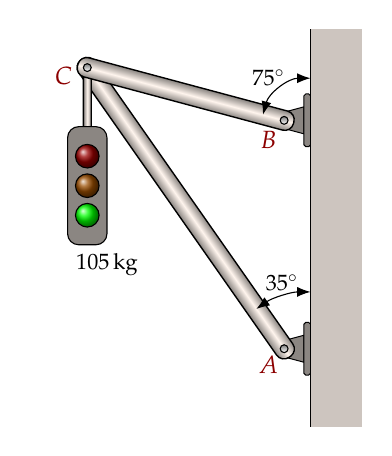
\begin{tikzpicture}[scale=0.5]

	\coordinate (C) at (0,0);
	\coordinate (B) at ($ (C)+(-15:5.176) $);
	\coordinate (A) at ($ (C)+(-55:8.717) $);
	\coordinate (D) at ($ (C)+(0,-3) $);

	\gettikzxy{(A)}{\ax}{\ay}
  \gettikzxy{(B)}{\bx}{\by}
  \gettikzxy{(C)}{\cx}{\cy}

	\PC[90]{B}{Seashell4}{black}{0.67}{0.125}
	\PC[90]{A}{Seashell4}{black}{0.67}{0.125}

	\fill[Seashell3] ($ (\bx+0.67cm, \cy+1cm) $) rectangle ($ (\ax+2cm, \ay-2cm) $);
	\draw[thin]  ($ (\bx+0.67cm, \cy+1cm) $) -- ($ (\bx+0.67cm, \ay-2cm) $);
	
	\Member{C}{A}{Seashell4}{Seashell1}{black}{0.5}{1.125}{0.5}	
	\Member{C}{D}{Seashell4}{Seashell1}{black}{0.2}{.125}{0.5}
	\Member{C}{B}{Seashell4}{Seashell1}{black}{0.5}{1.125}{0.5}

	\filldraw[rounded corners, fill=Seashell4] ($ (D)+(-0.5,-1.5) $) rectangle ($ (D)+(0.5,1.5) $);
	\shadedraw[ball color=orange!60!black] (D) circle (.3cm);
	\shadedraw[ball color=red!60!black] ($(D)+(0,0.75)$) circle (.3cm);
	\shadedraw[ball color=green] ($(D)+(0,-0.75)$) circle (.3cm);
	\node at ($ (D)-(-0.5,2) $) {\footnotesize $ 105\,$kg};

	\draw[Latex-Latex] ($ (B)+(-15:0.6936)+(0,1.25) $) arc (90:165:1.25) node[midway,xshift=-1.5mm, yshift=1.3mm] {\footnotesize $75\deg$};
	\draw[Latex-Latex] ($ (A)+(-55:1.168)+(0,2.4) $) arc (90:125:2.4) node[midway,yshift=1.75mm] {\footnotesize $35\deg$};

	\small
	
	\shadedraw [draw=black] (B) circle (0.1cm) node[statsMaroon, xshift=-0.2cm, yshift=-0.25cm] {$B$};
	\shadedraw [draw=black] (A) circle (0.1cm) node[statsMaroon, xshift=-0.2cm, yshift=-0.2cm] {$A$};
	\shadedraw [draw=black] (C) circle (0.1cm) node[statsMaroon, xshift=-0.3cm, yshift=-0.1cm] {$C$};

	\pgfresetboundingbox
	\draw[white] (\cx-1.5cm, \cy+1cm) rectangle (\ax+2cm, \ay-2cm);
	

\end{tikzpicture}



			}
			% \begin{center}
			% 	\footnotesize
			% 	\rotatebox[origin=c]{180}{
			% 		\textcolor{gray}{
			% 			($BC=919\text{ N}, AC=1.55\text{ kN}$)
			% 		}
			% 	}
			% \end{center}
		\end{myexam}
	}
\end{frame}

%%%%%%%%%%%%%%%%%%%%%%%%%%%%%%%%%%%%%%%%%%%%%%%%%%%%%%%%%%%%%%%%%%%%%%%%%%%%%%%%%%%
\begin{frame}{Component Forces}


	\begin{myexer}{}{}
		\centering
		\def\scale{0.675}
		\scalebox{0.675}{
			\tikz{%
  \coordinate (A) at (0,0);
  \coordinate (B) at (2.5,0);
  \coordinate (C) at (5.5,0);
  \coordinate (D) at (8,1.25);
  \coordinate (E) at (8,-3);
  \coordinate (F) at (5.5,-3);
  \coordinate (G) at (2.5,-3);

  \gettikzxy{(C)}{\Cx}{\Cy};
	\gettikzxy{(E)}{\Ex}{\Ey};
	\gettikzxy{(D)}{\Dx}{\Dy};

  \fill[AntiqueWhite3] ($ (E)+(0.5,-1) $) rectangle ($ (D)+(1.5,1.5) $);
	\draw[black, thick] ($ (E)+(0.5,-1) $) -- ($ (D)+(0.5,1.5) $);

  \PC[90]{D}{AntiqueWhite4}{black}{0.5}{0.25}
	\PC[90]{E}{AntiqueWhite4}{black}{0.5}{0.25}

  \Member{A}{B}{Cornsilk4}{white}{black}{0.3125}{1.5}{0.25}
  \Member{B}{C}{Cornsilk4}{white}{black}{0.3125}{1.5}{0.25}
  \Member{C}{D}{Cornsilk4}{white}{black}{0.3125}{1.5}{0.25}
  \Member{E}{F}{Cornsilk4}{white}{black}{0.3125}{1.5}{0.25}
  \Member{F}{G}{Cornsilk4}{white}{black}{0.3125}{1.5}{0.25}
  \Member{A}{G}{Cornsilk4}{white}{black}{0.3125}{1.5}{0.25}
  \Member{C}{G}{Cornsilk4}{white}{black}{0.3125}{1.5}{0.25}
  \Member{C}{E}{Cornsilk4}{white}{black}{0.3125}{1.5}{0.25}
  \Member{B}{G}{Cornsilk4}{white}{black}{0.3125}{1.5}{0.25}
  \Member{C}{F}{Cornsilk4}{white}{black}{0.3125}{1.5}{0.25}

  \draw[thin, black] ($ (A)+(0,0.325)$) -- +(0,2.25);
  \draw[thin, black] ($ (B)+(0,0.325)$) -- +(0,2.25);
  \draw[thin, black] ($ (C)+(0,0.325)$) -- +(0,2.25);
  \draw[thin, black] ($ (D)+(0,0.325)$) -- +(0,1);
  \draw[thin, black] ($ (D)+(0.25,0)$) -- +(2.25,0);
  \draw[thin, black] ($ (E)+(0.25,0)$) -- +(2.25,0);
  \draw[thin, black] ($ (C)+(0.5,0)$) -- +(4.5,0);

  \draw[thick, latex-latex] ([yshift=2.125cm]A) -- node[fill=white, inner sep=0.375mm]{$2.50$ m}([yshift=2.125cm]B);
	\draw[thick, latex-latex] ([yshift=2.125cm]B) -- node[fill=white, inner sep=0.375mm]{$3.00$ m}([yshift=2.125cm]C);
	\draw[thick, latex-latex] ([yshift=2.125cm]C) -- node[fill=white, inner sep=0.375mm]{$2.50$ m}([yshift=0.875cm]D);
	\draw[thick, latex-latex] (10.125, \Dy) -- node[fill=white, inner sep=0.75mm]{$1.25$ m}(10.125, \Cy);
	\draw[thick, latex-latex] (10.125, \Cy) -- node[fill=white, inner sep=0.75mm]{$3.00$ m}(10.125, \Ey);


  \draw[line width=0.625mm, statsMaroon, -Latex, line cap=round] (A) -- +(0,-2.5) node[below] {\Large {$\bm{4.20}$ \bf kN}};

  \fill[ball color=AntiqueWhite4] (A) circle (3pt) node[above left, inner sep=2mm] {\large $\bm A$};
	\fill[ball color=AntiqueWhite4] (B) circle (3pt) node[above left, inner sep=2mm] {\large $\bm B$};
	\fill[ball color=AntiqueWhite4] (C) circle (3pt) node[above left, inner sep=2mm] {\large $\bm C$};
	\fill[ball color=AntiqueWhite4] (D) circle (3pt) node[above left, inner sep=1.5mm] {\large $\bm D$};
	\fill[ball color=AntiqueWhite4] (E) circle (3pt) node[below left, inner sep=2.5mm] {\large $\bm E$};
	\fill[ball color=AntiqueWhite4] (F) circle (3pt) node[below left, inner sep=2mm] {\large $\bm F$};
	\fill[ball color=AntiqueWhite4] (G) circle (3pt) node[below left, inner sep=2mm] {\large $\bm G$};


  % \pgfresetboundingbox
  \useasboundingbox ($ (A)+ (-0.75,3) $) rectangle ($ (E)+(2.875,-1.25) $);





}
		}
		\parm
		\cmini[0.9]{
			Resolve the $4.20$ kN load suspended from $A$ into components parallel to the truss members $AB$ and $AG$. Give the magnitude of the components and their direction measured counter-clockwise from the positive $x$ axis.
		}


		% \begin{center}
		% 	\footnotesize
		% 	\rotatebox[origin=c]{180}{
		% 		\textcolor{gray}{
		% 			($35.0\text{ kN at } 180^\circ, 54.7\text{ kN at} 310^\circ $)
		% 		}
		% 	}
		% \end{center}
	\end{myexer}

\end{frame}

%%%%%%%%%%%%%%%%%%%%%%%%%%%%%%%%%%%%%%%%%%%%%%%%%%%%%%%%%%%%%%%%%%%%%%%%%%%%%%%%

\begin{frame}{Component Forces}
	\cmini[1]{
		\begin{myexer}[bottom=0mm]{}{}
			\mini[0.4]{
				\raggedright
				The decoration suspended at $D$ weighs $1124\,\mathsf{N}$.\parm 
				Determine the magnitudes of the two force components of the weight of $D$, in the direction of $AB$ and $BC$.
			}
			\hfill
			\mini[0.5]{
				\centering
				\def\scale{0.7}
				
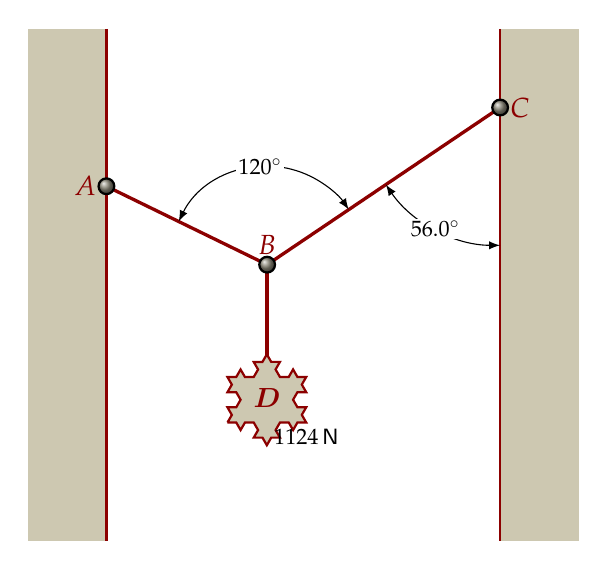
\begin{tikzpicture}[scale=\scale, decoration=Koch snowflake,draw=statsMaroon,fill=Cornsilk3,thick]

	\coordinate (A) at (0,-2);
	\coordinate (AA) at ($(A)+(-26:1)$);
	\coordinate (C) at (5,-1);
	\coordinate (CC) at ($(C)+(214:1)$);
	\coordinate (B) at (intersection of A--AA and C--CC);
	\coordinate (D) at ($ (B)+(0,-1.6875) $);

	\fill[Cornsilk3] ($ (A)+(0,2) $) rectangle  ($ (A)+(-1,-4.5) $); 
	\fill[Cornsilk3] ($ (C)+(0,1) $) rectangle  ($ (C)+(1,-5.5) $); 
	\draw[thick, statsMaroon] ($ (A)+(0,2) $) -- ($ (A)+(0,-4.5) $); 
	\draw[thick, statsMaroon] ($ (C)+(0,1) $) -- ($ (C)+(0,-5.5) $); 


	\draw[very thick, statsMaroon] (A)--(B);
	\draw[very thick, statsMaroon] (B)--(C);
	\draw[very thick, statsMaroon] (B)--(D);

	\filldraw[xshift=1.5375cm, yshift=-2.5cm] decorate{ decorate{ (0,-2.5) -- ++(60:1) -- ++(-60:1) -- cycle }};


	\draw[black, thin, latex-latex] ($ (B)+(154:1.25) $) arc (154:34:1.25) node[fill=white, inner sep=0.25mm, midway] {\footnotesize $120\deg$};
	\draw[black, thin, latex-latex] ($ (C)+(270:1.75) $) arc (270:214:1.75) node[fill=white, inner sep=0.25mm, midway] {\footnotesize $56.0\deg$};


	\shadedraw [draw=black, ball color = Cornsilk4] (B) circle (0.1cm) node[statsMaroon,above] {$B$};
	\shadedraw [draw=black, ball color = Cornsilk4] (A) circle (0.1cm) node[statsMaroon, left] {$A$};
	\shadedraw [draw=black, ball color = Cornsilk4] (C) circle (0.1cm) node[statsMaroon, right] {$C$};
	\node[statsMaroon] at (D) {$\bm D$};
	\node[black, xshift=0.5cm, yshift=-0.5cm] at (D) {\footnotesize $1124\,\mathsf{N}$};



\end{tikzpicture}

			}
			% \begin{center}
			% 	\footnotesize
			% 	\rotatebox[origin=c]{180}{
			% 		\textcolor{gray}{
			% 			($1170$ kN along $AB$ and $1080$ kN along $BC$)
			% 		}
			% 	}
			% \end{center}
		\end{myexer}
	}

\end{frame}
%%%%%%%%%%%%%%%%%%%%%%%%%%%%%%%%%%%%%%%%%%%%%%%%%%%%%%%%%%%%%%%%%%%%%%%%%%%%%%%%

\begin{frame}{Resultant \& Component Forces}
	
		\begin{myexam}{}{}
			\mini[0.55]{
				\begin{enumerate}[{a)}]
					\item Determine the resultant ${\bm R}$ of the two vectors ${\bm F}$ and ${\bm G}$.
					\item Determine the $x$-component of ${\bm R }$ (i.e., the horizontal component).
					\item Determine the $x$-component of ${\bm F }$.
					\item Determine the $x$-component of ${\bm  G }$.
					\item Add the two previous results. Compare it with the result from $\color{statsMaroon}b)$ above.
				\end{enumerate}
			}
			\hfill
			\mini[0.35]{
				
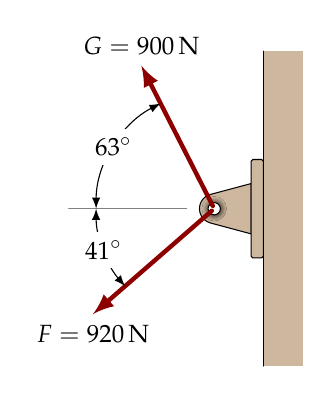
\begin{tikzpicture}[scale=\scale, line cap = round]

	\coordinate (A) at (0,0);

	\EyeConnection[90]{A}{Bisque3}{black}{0.625}{0.375}
	\fill[Bisque3] ($ (A)+(0.625,2) $) rectangle ($ (A)+(1.125,-2) $);
	\draw ($ (A)+(0.625,2) $) -- ($ (A)+(0.625,-2) $);

	\draw[ultra thick, statsMaroon, -latex] ($ (A)+(117:0.04) $) -- +(117:2) node[black, yshift=0.25cm] {\small $ G=900\,$N};
	\draw[ultra thick, statsMaroon, -latex] ($ (A)+(221:0.04) $) -- +(221:2) node[black, yshift=-0.25cm] {\small $ F=920\,$N};

	\draw[gray] ($ (A)-(0.35cm,0) $) -- +(-1.5,0);

	\draw[latex-latex] ($ (A)+(117:1.5) $) arc (117:180:1.5) node[midway, fill=white] {\small $ 63\deg $};
	\draw[latex-latex] ($ (A)+(221:1.5) $) arc (221:180:1.5) node[midway, fill=white] {\small $ 41\deg $};


\end{tikzpicture}

			}
		\end{myexam}	

\end{frame}

%%%%%%%%%%%%%%%%%%%%%%%%%%%%%%%%%%%%%%%%%%%%%%%%%%%%%%%%%%%%%%%%%%%%%%%%%%%%%%%%

%%%%%%%%%%%%%%%%%%%%%%%%%%%%%%%%%%%%%%%%%%%%%%%%%%%%%%%%%%%%%%%%%%%%%%%%%%%%%%%%

\begin{frame}{Resultant \& Component Forces}

	
		\begin{myexer}{}{}
			\mini[0.5]{
				\begin{enumerate}[{a)}]
					\item Determine the magnitude of the component of ${\bm R }$ (found in the previous example) along the $y-$axis (i.e., the vertical component).
					\item Determine the magnitude of the component of ${\bm F }$ along the $y$ axis.
					\item Determine the magnitude of the component of ${\bm G }$ along the $y$ axis.
					\item Add the two previous results.
				\end{enumerate}
			} % end mini
			\hfill
			\mini[0.35]{
				
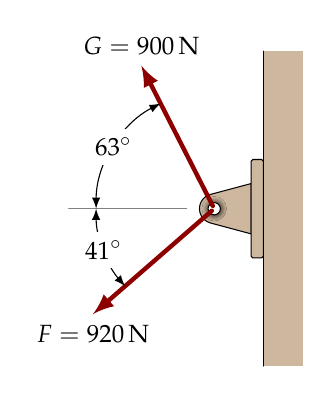
\begin{tikzpicture}[scale=\scale, line cap = round]

	\coordinate (A) at (0,0);

	\EyeConnection[90]{A}{Bisque3}{black}{0.625}{0.375}
	\fill[Bisque3] ($ (A)+(0.625,2) $) rectangle ($ (A)+(1.125,-2) $);
	\draw ($ (A)+(0.625,2) $) -- ($ (A)+(0.625,-2) $);

	\draw[ultra thick, statsMaroon, -latex] ($ (A)+(117:0.04) $) -- +(117:2) node[black, yshift=0.25cm] {\small $ G=900\,$N};
	\draw[ultra thick, statsMaroon, -latex] ($ (A)+(221:0.04) $) -- +(221:2) node[black, yshift=-0.25cm] {\small $ F=920\,$N};

	\draw[gray] ($ (A)-(0.35cm,0) $) -- +(-1.5,0);

	\draw[latex-latex] ($ (A)+(117:1.5) $) arc (117:180:1.5) node[midway, fill=white] {\small $ 63\deg $};
	\draw[latex-latex] ($ (A)+(221:1.5) $) arc (221:180:1.5) node[midway, fill=white] {\small $ 41\deg $};


\end{tikzpicture}

			}
		\end{myexer}

\end{frame}
%%%%%%%%%%%%%%%%%%%%%%%%%%%%%%%%%%%%%%%%%%%%%%%%%%%%%%%%%%%%%%%%%%%%%%%%%%%%%%%%

\begin{frame}{Rectangular Components}
	\mini[0.9]{
		\raggedright
		When a force vector, $\bm F$, is resolved into horizontal and vertical components (i.e., along the $x$-axis and the $y$-axis), they are referred to as {\bf rectangular components} (or $x$ and $y$-components). 
	}
	\parm
	
	\mini[0.35]{
		\begin{statsbox}{}
			% !TEX root = ../../statikz/statikz.tex


\begin{tikzpicture}[scale = 0.5, style={line cap = round}]
  
  \draw (-0.75,0) -- (4.75,0) node[right] {$x$};  
  \draw (0, -0.75) -- (0, 4.75) node[above] {$y$};  
  \draw[ultra thick, saitMaroon, -latex] (0, 0) -- (3, 4) node [above right, black] {\large $\bm F $};
  \draw[latex-latex] (1.5cm, 0.5mm) arc[start angle = 0, end angle = 51, radius = 1.5cm];
  \node [right] at (1.25, 0.9) {$\theta$};
  \draw[white] (-1.25,-1.25) rectangle (5.75, 5.5);

  \only<2>{
    \draw[ultra thick, black, -latex] (0, 0) -- node [below] {\large $\bm{F_x }$} ++(3, 0) ;
    \draw[ultra thick, black, -latex] (0, 0) --  node [left] {\large $\bm{F_y }$} ++(0, 4);
  }

  \only<2->{
  \draw[Gainsboro] (0, 4) -- (3, 4);
  \draw[Gainsboro] (3, 0) -- (3, 4);
  
  }

  \only<3->{
    \draw[ultra thick, black, -latex] (0, 0) -- node [below] {\large $\bm{\mathrm{F}_x }$} ++(3, 0) ;
    \draw[ultra thick, black, -latex] (0, 0) --  node [left] {\large $\bm{\mathrm{F}_y }$} ++(0, 4);
  }

  
  
\end{tikzpicture}

		\end{statsbox}
	}
	\hfill
	\mini[0.6]{
		\begin{itemize}
			\item<2->  Force $\bm F $  is resolved into component vectors $\bm {F _x}$  and $\bm {F_y}$ along the $x$ and $y$-axes. $$ \bm{ F = F_x + F_y} $$
			\item<3-> We know the directions of the component vectors (along the axes) so we are generally only interested in the magnitude of these vectors, which is a scalar value. The magnitudes of  $\bm{F_x}$  and $\bm{F_y}$ are given by the scalar values:
			      $$ \bm{\mathrm{F}_x=\lvert F\rvert \cd\cos\theta \text{ and } \mathrm{F}_y=\lvert F\rvert\cd\sin\theta} $$
						where $\lvert F\rvert$ is the length/magnitude of $F$.
			\item<4-> Rectangular components along the negative axes have negative scalar values.
		\end{itemize}
	}
\end{frame}


%%%%%%%%%%%%%%%%%%%%%%%%%%%%%%%%%%%%%%%%%%%%%%%%%%%%%%%%%%%%%%%%%%%%%%%%%%%%%%%%

%%%%%%%%%%%%%%%%%%%%%%%%%%%%%%%%%%%%%%%%%%%%%%%%%%%%%%%%%%%%%%%%%%%%%%%%%%%%%%%%

\begin{frame}{Rectangular Components: Signs by Quadrant}
	\centering
	% !TEX root = ../../statikz/statikz.tex

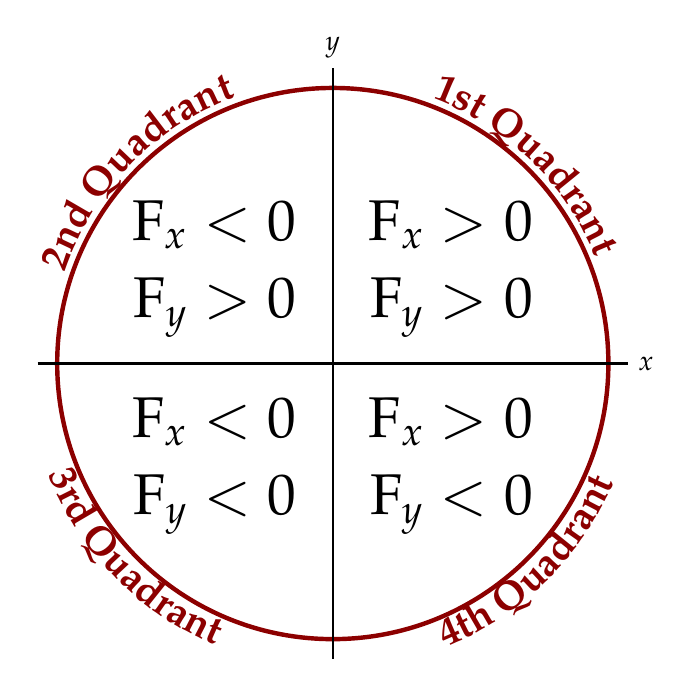
\begin{tikzpicture}
  \filldraw [white, draw=saitMaroon, ultra thick ] (0, 0) circle (3.5cm);
  \draw[thick, black] (-3.75,0) -- (3.75, 0) node [right] {$x$};
  \draw[thick, black] (0, -3.75) -- (0, 3.75) node [above] {$y$};

  \path[decorate, decoration={text along path, text={|\color{saitMaroon}\Large\bf|1st Quadrant||\ }, text align = center}] (0, 3.6) arc (90:0:3.6);

  \path[decorate, decoration={text along path, text={|\color{saitMaroon}\Large\bf|2nd Quadrant||\ }, text align = center}] (-3.6, 0) arc (180:90:3.6);

  \path[decorate, decoration={text along path, text={|\color{saitMaroon}\Large\bf|3rd Quadrant||\ }, text align = center}] (-3.875, 0) arc (180:270:3.875);

  \path[decorate, decoration={text along path, text={|\color{saitMaroon}\Large\bf|4th Quadrant||\ }, text align = center}] (0, -3.875) arc (270:360:3.875);

  \node at (1.5, 1.25) {\huge $ \begin{aligned}{\mathrm{F}_x} &>0\\\mathrm{F}_y &>0\end{aligned} $};
  \node at (-1.5, 1.25) {\huge $ \begin{aligned}\mathrm{F}_x &<0\\\mathrm{F}_y &>0\end{aligned} $};
  \node at (-1.5, -1.25) {\huge $ \begin{aligned}\mathrm{F}_x &<0\\\mathrm{F}_y &<0\end{aligned} $};
  \node at (1.5, -1.25) {\huge $ \begin{aligned}\mathrm{F}_x &>0\\\mathrm{F}_y &<0\end{aligned} $};

\end{tikzpicture}

\end{frame}

%%%%%%%%%%%%%%%%%%%%%%%%%%%%%%%%%%%%%%%%%%%%%%%%%%%%%%%%%%%%%%%%%%%%%%%%%%%%%%%%

\begin{frame}{Rectangular Components}

	\begin{myexam}{}{}
		\mini[0.5]{
			% !TEX root = ../../statikz/statikz.tex

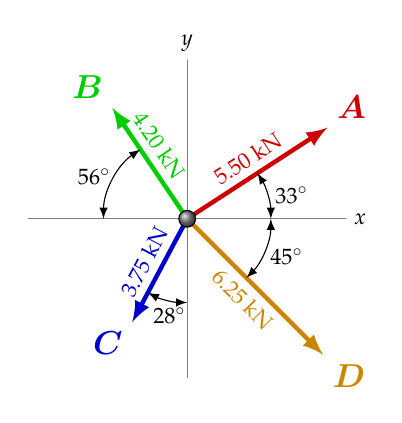
\begin{tikzpicture}[scale = 0.425, style={line cap = round}]
  \footnotesize
  \draw[gray] (-4.75,0) -- (4.75,0) node[right, black] {$x$};
  \draw[gray] (0, -4.75) -- (0, 4.75) node[above, black] {$y$};

  \draw[ultra thick, Red3, -latex] (0, 0) -- node[above, sloped]{$5.50$ kN} ++(33:5cm) node [above right] {\large $\bm A $};
  \draw[latex-latex] (2.5cm, 0mm) arc[start angle = 0, end angle = 33, radius = 2.5cm];
  \node [right] at (2.4, 0.7) { $33\deg$};

  \draw[ultra thick, Green3, -latex] (0, 0) -- node[above, sloped, xshift=-0.125cm]{\footnotesize $4.20$ kN} ++(124:4cm) node [above left] {\large $ \bm B $};
  \draw[latex-latex] (-2.5cm, 0mm) arc[start angle = 180, end angle = 124, radius = 2.5cm];
  \node [right] at (-3.5, 1.25) { $56\deg$};

  \draw[ultra thick, Blue3, -latex] (0, 0) -- node[above, sloped]{ $3.75$ kN} ++(242:3.5cm) node [below left] {\large $\bm C $};
  \draw[latex-latex] (0, -2.5cm) arc[start angle = 270, end angle = 242, radius = 2.5cm];
  \node [right] at (-1.25, -2.9) { $28\deg$};

  \draw[ultra thick, Orange3, -latex] (0, 0) -- node[below, sloped]{ $6.25$ kN} ++(-45:5.75cm) node [below right] {\large $\bm D $};
  \draw[latex-latex] (2.5cm, 0) arc[start angle = 0, end angle = -45, radius = 2.5cm];
  \node [right] at (2.25, -1.15) { $45\deg$};

  \shadedraw[ball color=gray] (0,0) circle (0.25cm);

\end{tikzpicture}

		}
		\hfill
		\mini[0.45]{
			\small

			Find the rectangular components of each of  $\bm A$, $\bm B$, $\bm C$ and $\bm D$.

			\mini[0.8]{

				\uncover<2->{
					\color{Red3}
					\begin{align*}
						\mathrm{A}_x & = 5.50\cos 33\deg\text{ kN} = 4.61\text{ kN} \\
						\mathrm{A}_y & = 5.50\sin 33\deg\text{ kN} = 3.00\text{ kN}
					\end{align*}
				}
				\uncover<3->{
					\color{Green3}
					\vspace{-0.5cm}
					\begin{align*}
						\mathrm{B}_x & = -4.20\cos 56\deg\text{ kN} = -2.35\text{ kN} \\
						\mathrm{B}_y & = 4.20\sin 56\deg\text{ kN} = 3.48\text{ kN}
					\end{align*}
				}
				\uncover<4->{
					\color{Blue3}
					\vspace{-0.5cm}
					\begin{align*}
						\mathrm{C}_x & = -3.75\sin 28\deg\text{ kN}= -1.761\text{ kN} \\
						\mathrm{C}_y & = -3.75\cos 28\deg\text{ kN} = -3.31\text{ kN}
					\end{align*}
				}
				\uncover<5->{
					\color{Orange3}
					\vspace{-0.5cm}
					\begin{align*}
						\mathrm{D}_x & = 6.25\cos 45\deg\text{ kN}  = 4.42\text{ kN}  \\
						\mathrm{D}_y & = -6.25\cos 45\deg\text{ kN} = -4.42\text{ kN}
					\end{align*}
				}
			}
		}
	\end{myexam}

\end{frame}

%%%%%%%%%%%%%%%%%%%%%%%%%%%%%%%%%%%%%%%%%%%%%%%%%%%%%%%%%%%%%%%%%%%%%%%%%%%%%%%%

\begin{frame}{Force Resultants using Rectangular Components}


	\cmini[0.8]{
		To determine the resultant of several forces:\parb
		\begin{enumerate}
			\item Resolve each force into its $x$ and $y$-components.
			\item Sum the $x$ components, $\Sigma \mathrm{F}_x$.
			\item Thenk $\Sigma \mathrm{F}_x = \mathrm{R}_x$, the $x$-component of the resultant.
			\item Similarly, sum the $y$ components, $\Sigma \mathrm{F}_y$, to find $\mathrm{R}_y$, the $y$-component of the resultant.
			\item From the $\mathrm{R}_x$ and $\mathrm{R}_y$, determine the magnitude and direction of the resultant vector.
		\end{enumerate}
		\parb
		This process makes finding the resultant of more than two forces much simpler than repeated applications of the triangle or parallelogram laws.
	}

\end{frame}
%%%%%%%%%%%%%%%%%%%%%%%%%%%%%%%%%%%%%%%%%%%%%%%%%%%%%%%%%%%%%%%%%%%%%%%%%%%%%%%%

\begin{frame}{From Rectangular Components to the Resultant Components}
	\begin{myexam}{}{}
		\mini[0.5]{

			% !TEX root = ../../Beamer/02ForceVectors/02ForceVectors.tex

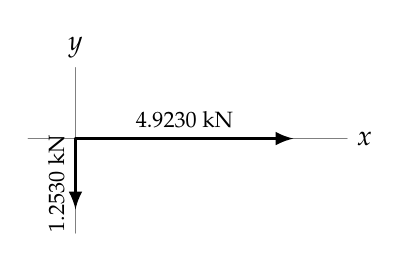
\begin{tikzpicture}[scale = 0.6, style={line cap = round}]
	
	\draw[gray](-1,0) -- (5.75,0) node[black, right] {$x$};
	\draw[gray] (0, -2) -- (0, 1.5) node[black, above] {$y$};
	\uncover<2->{
		\draw[very thick, -latex] (0, 0) -- node[above, sloped]{\footnotesize $4.9230$ kN} (4.613, 0);
	}
	\uncover<3->{
		\draw[very thick, latex-] (0, -1.5) -- node[above, xshift=-0.125cm, sloped]{\footnotesize $1.2530$ kN}  (0, 0);
	}

	%  \draw[<->] (2.5cm, 0mm) arc[start angle = 0, end angle = 33, radius = 2.5cm];
	%  \node [rectangle, right] at (2.4, 0.7) {\small $33\degree$};
	% \uncover<2->{
	%   \draw (0, -1.253) -- (4.613, -1.253) -- (4.613, 0);
	% }
	% \uncover<3->{
	%   \draw[very thick, saitRed, ->, >=stealth] (0, 0) -- node[above, sloped, very near end]{\footnotesize $\bm{\mathrm{ F }_{R}}$}(4.613, -1.253);
	%   \draw[<->] (2, 0)  arc[start angle = 0, end angle = -15.2, radius = 2cm] ;
	%   \node at (2.2, -0.3) {\footnotesize $\theta$};
	% }
\end{tikzpicture}

		}
		\hfill
		\mini[0.45]{
			\small\raggedright
			
			Find the rectangular components of $\bm R$, where $\bm R$ is the resultant of forces $\bm A$, $\bm B$, $\bm C$ and $\bm D$ from the previous example.
		
			\uncover<2->{
				\begin{align*}
					R_x & = \Sigma F_x                              \\
							& = 4.6127\text{ kN} - 2.3486\text{ kN}     \\
							& \qquad -1.7605\text{ kN}+4.4194\text{ kN} \\
							& = 4.9230\text{ kN}
				\end{align*}				
			}
			\uncover<3>{
				\begin{align*}
					R_y & = \Sigma F_y                              \\
							& = 2.9955\text{ kN} + 3.4820\text{ kN}     \\
							& \qquad -3.3111\text{ kN}-4.4194\text{ kN} \\
							& = -1.2530\text{ kN}
				\end{align*}
			}
		}			
	
	\end{myexam}
\end{frame}

%%%%%%%%%%%%%%%%%%%%%%%%%%%%%%%%%%%%%%%%%%%%%%%%%%%%%%%%%%%%%%%%%%%%%%%%%%%%%%%%

\begin{frame}{The Resultant, From its Components}
	\begin{myexam}{}{}
		\mini[0.5]{
			\begin{enumerate}
				\item<1-> Draw the components. (Negative components are drawn along the negative axes.)
				\item<2-> Form a rectangle.
				\item<3-> Draw the resultant (the diagonal of the rectangle, starting at the origin).
			\end{enumerate}

		}
		\hfill
		\mini[0.45]{
			% !TEX root = ../../Beamer/02ForceVectors/02ForceVectors.tex

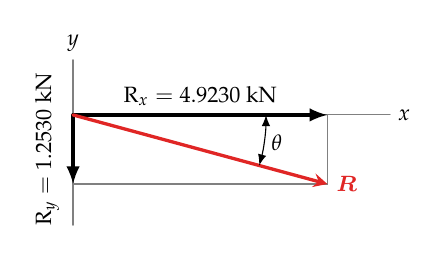
\begin{tikzpicture}[scale = 0.7, style={line cap = round}]
 \footnotesize
  \only<1->{
  \draw[gray](0,0) -- (5.75,0) node[black, right] {$x$};
  \draw[gray] (0, -2) -- (0, 1) node[black, above] {$y$};
  }

  \draw[very thick, -latex] (0, 0) -- node[above, sloped]{\footnotesize $\mathrm{R}_x=4.9230$ kN} (4.613, 0);
  \draw[very thick, latex-] (0, -1.253) -- node[above, sloped, yshift=0.0625cm]{\footnotesize $\mathrm{R}_y=1.2530$ kN}  (0, 0);
  %  \draw[<->] (2.5cm, 0mm) arc[start angle = 0, end angle = 33, radius = 2.5cm];
  %  \node [rectangle, right] at (2.4, 0.7) {\small $33\degree$};
  \uncover<2->{
    \draw[gray] (0, -1.253) -- (4.613, -1.253) -- (4.613, 0);
  }
  \uncover<3->{
    \draw[very thick, saitRed, ->, >=stealth] (0, 0) -- (4.613, -1.253)node[right]{\footnotesize $\bm{R}$};
    \draw[latex-latex] (3.5, 0)  arc[start angle = 0, end angle = -15.2, radius = 3.5cm] ;
    \node at (3.7, -0.5) {\footnotesize $\theta$};
  }
\end{tikzpicture}

		}
		\vspace{0.125cm}
		\begin{enumerate}
			\setcounter{enumi}{3}
			\item<4-> The magnitude of the resultant is given by \footnotesize
			$$ \bm{ \lvert R \rvert }= \sqrt{(4.9230\text{ kN})^2+(1.2530\text{ kN})^2} = 5.0800 \text{ kN} = \bm{5.08\text{ \bfseries kN}}$$
			\item<5-> The direction of the resultant is given by \footnotesize
			$$  \bm\theta = \tan^{-1}\frac{\lvert \mathrm{R}_y\rvert}{\left|\mathrm{R}_x\right|}=\tan^{-1}\left[\frac{1.2530}{4.9230}\right] = 14.280^\circ = \bm{14.3^\circ}$$
		\end{enumerate}
		\vspace{-0.5cm}
	\end{myexam}
	\uncover<6>{ \small\centering

		\tcb{%
			${\bm R}$ is $5.08\text{ kN}$ at $14.3\deg $, measure clockwise from the positive $x$-axis.		
		}
	}
\end{frame}
%%%%%%%%%%%%%%%%%%%%%%%%%%%%%%%%%%%%%%%%%%%%%%%%%%%%%%%%%%%%%%%%%%%%%%%%%%%%%%%%

\begin{frame}	
	\cmini[0.9]{
		\begin{myexam}{}{}

			\cmini{
				\def\scale{0.8}
				\centering
				
% !TEX root = ../../Beamer/02ForceVectors/02ForceVectors.tex


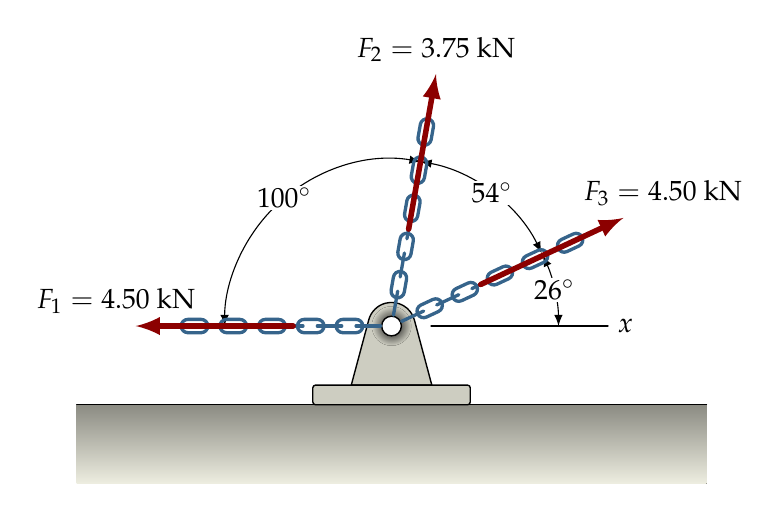
\begin{tikzpicture}[scale=\scale, line cap=round,decoration={
		markings,% switch on markings
		mark=% actually add a mark
		between positions 0 and 1 step 14pt
		with
		{
			\begin{scope}[scale=0.8]
				\draw[SteelBlue4, very thick] (0pt,-3pt) -- ++(6pt,0) arc(-90:90:3pt) -- ++(-6pt,0pt) arc(90:270:3pt) -- cycle;
				\draw[SteelBlue4,very thick] (-11pt,0) -- (0pt,0);
			\end{scope}
		}
	}]

	\coordinate (D) at (-3,1);
	\coordinate (E) at (3, 2.5);
	\coordinate (C) at (0, 0);

\begin{scope}
	\fill[top color=Ivory4, bottom color=Ivory2] (-4,-1) rectangle (4,-2);
	\draw[thin, black] (-4,-1) -- ($(4,-2.5)+(0,1.5) $);
	\EyeConnection{C}{Ivory3}{black}{1}{0.5}
\end{scope}

	\draw[latex-latex] ($ (C)+(26:2.12)$) arc (26:80:2.12) node[fill=white, midway, inner sep=0.25mm] {$54^\circ$};
	\draw[latex-latex] ($ (C)+(0:2.12)$) arc (0:25:2.12) node[fill=white, midway, inner sep=0.25mm] {$ 26^\circ $};
	\draw[latex-latex] ($ (C)+(80:2.12)$) arc (80:180:2.12) node[fill=white, midway, inner sep=0.25mm] {$ 100^\circ $};


	\path[postaction={decorate}] ($ (C)+(25:0.45) $) -- +(25:2);
	\path[postaction={decorate}] ($ (C)+(180:0.45) $) -- +(180:2);
	\path[postaction={decorate}] ($ (C)+(80:0.45) $) -- +(80:2);
	\draw[line width=2pt, -latex, saitMaroon] ($ (C)+(180:1.25) $) -- +(180:2) node[xshift=-0.25cm, black, above]{$ F_1=4.50 $ kN};
	\draw[line width=2pt, -latex, saitMaroon] ($ (C)+(80:1.25) $) -- +(80:2) node[black, above]{$F_2=3.75 $ kN};
	\draw[line width=2pt, -latex, saitMaroon] ($ (C)+(25:1.25) $) -- +(25:2) node[xshift=0.5cm, black, above]{$F_3=4.50 $ kN};



	\draw[thin] ($(C)+(0.5,0) $) -- +(2.25,0) node[right] {$x$};




\end{tikzpicture}

			}
			Determine the resultant (magnitude and direction counterclockwise from the positive $x$ axis) of the three forces $F_1,\;F_2$ and $F_3$ acting at a single point.
		% 	\parm
		% 	\begin{center}
		% 		\footnotesize
		% 		\rotatebox[origin=c]{180}{
		% 			\textcolor{gray}{
		% 				($5.67$ kN at $88.0\deg$)
		% 			}
		% 		}
		% 	\end{center}
		\end{myexam}
	}
	

\end{frame}

%%%%%%%%%%%%%%%%%%%%%%%%%%%%%%%%%%%%%%%%%%%%%%%%%%%%%%%%%%%%%%%%%%%%%%%%%%%%%%%%

\begin{frame}

	% centered minipage with text raggedright
	%cmini[width]{content}
	\cmini[0.9]{
		\begin{myexam}{}{}
			\def\scale{0.7}
			\cmini{
				\centering
				
% !TEX root = ../../Beamer/02ForceVectors/02ForceVectors.tex


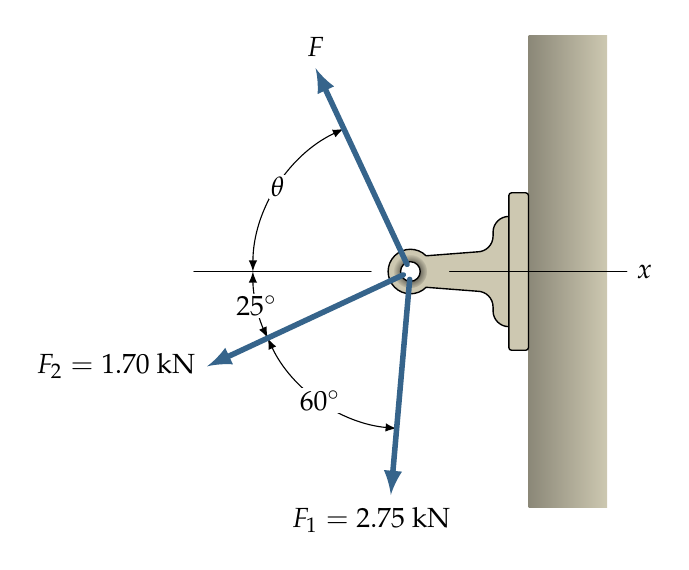
\begin{tikzpicture}[scale=\scale, line cap=round,decoration={
		markings,% switch on markings
		mark=% actually add a mark
		between positions 0 and 1 step 14pt
		with
		{
			\begin{scope}[scale=0.8]
				\draw[SteelBlue4, very thick] (0pt,-3pt) -- ++(6pt,0) arc(-90:90:3pt) -- ++(-6pt,0pt) arc(90:270:3pt) -- cycle;
				\draw[SteelBlue4,very thick] (-11pt,0) -- (0pt,0);
			\end{scope}
		}
	}]

	\coordinate (D) at (-3,1);
	\coordinate (E) at (3, 2.5);
	\coordinate (C) at (0, 0);

\begin{scope}
	\fill[left color = Cornsilk4, right color=Cornsilk3] (1.5,-3) rectangle (2.5,3);
	% \draw[thin, black] (-3,-1) -- ($(3,-2.5)+(0,1.5) $);
	\EyeBolt[90]{C}{Cornsilk3}{black}{1}{0.5}
\end{scope}

	\draw[latex-latex] ($ (C)+(115:2) $) arc (115:180:2) node[fill=white, midway, inner sep=0.25mm] {$\theta $};
	\draw[latex-latex] ($ (C)+(180:2) $) arc (180:205:2) node[fill=white, midway, inner sep=0.25mm] {$ 25\deg $};
	\draw[latex-latex] ($ (C)+(205:2) $) arc (205:265:2) node[fill=white, midway, inner sep=0.25mm] {$ 60\deg $};



	\draw[line width=2pt, -latex, SteelBlue4] ($ (C)+(-95:0.1) $) -- +(-95:2.75) node[xshift=-0.25cm, black, below]{$ F_1=2.75 $ kN};
	\draw[line width=2pt, -latex, SteelBlue4] ($ (C)+(115:.1) $) -- +(115:2.75) node[black, above]{$F$};
	\draw[line width=2pt, -latex, SteelBlue4] ($ (C)+(205:.1) $) -- +(205:2.75) node[black, left]{$F_2=1.70 $ kN};



	\draw[thin] ($(C)+(0.5,0) $) -- +(2.25,0) node[right] {$x$};
	\draw[thin] ($(C)+(-0.5,0) $) -- +(-2.25,0);




\end{tikzpicture}

			}
			\cmini{
				\raggedright
				The resultant of the forces $F,\;F_1$ and $F_2$ acting upon the eye-bolt is $30.7$ kN at $197^\circ$ measured counter-clockwise from the positive $x$ axis. \parm
				\centering Determine $F$ and $\theta$.
				% {\footnotesize
				% 	\rotatebox[origin=c, y=2.5pt]{180}{
				% 		\textcolor{gray}{
				% 			($F=28.1$ kN, $\theta=65.7^\circ$)
				% 		}
				% 	}
				% }
			}
		
		\end{myexam}
	}

\end{frame}

%%%%%%%%%%%%%%%%%%%%%%%%%%%%%%%%%%%%%%%%%%%%%%%%%%%%%%%%%%%%%%%%%%%%%%%%%%%%%%%%
%%%%%%%%%%%%%%%%%%%%%%%%%%%%%%%%%%%%%%%%%%%%%%%%%%%%%%%%%%%%%%%%%%%%%%%%%%%%%%%%
%%%%%%%%%%%%%%%%%%%%%%%%%%%%%%%%%%%%%%%%%%%%%%%%%%%%%%%%%%%%%%%%%%%%%%%%%%%%%%%%
%%%%%%%%%%%%%%%%%%%%%%%%%%%%%%%%%%%%%%%%%%%%%%%%%%%%%%%%%%%%%%%%%%%%%%%%%%%%%%%%
%%%%%%%%%%%%%%%%%%%%%%%%%%%%%%%%%%%%%%%%%%%%%%%%%%%%%%%%%%%%%%%%%%%%%%%%%%%%%%%%
%%%%%%%%%%%%%%%%%%%%%%%%%%%%%%%%%%%%%%%%%%%%%%%%%%%%%%%%%%%%%%%%%%%%%%%%%%%%%%%%
%%%%%%%%%%%%%%%%%%%%%%%%%%%%%%%%%%%%%%%%%%%%%%%%%%%%%%%%%%%%%%%%%%%%%%%%%%%%%%%%
%%%%%%%%%%%%%%%%%%%%%%%%%%%%%%%%%%%%%%%%%%%%%%%%%%%%%%%%%%%%%%%%%%%%%%%%%%%%%%%%
%%%%%%%%%%%%%%%%%%%%%%%%%%%%%%%%%%%%%%%%%%%%%%%%%%%%%%%%%%%%%%%%%%%%%%%%%%%%%%%%
%%%%%%%%%%%%%%%%%%%%%%%%%%%%%%%%%%%%%%%%%%%%%%%%%%%%%%%%%%%%%%%%%%%%%%%%%%%%%%%%
%%%%%%%%%%%%%%%%%%%%%%%%%%%%%%%%%%%%%%%%%%%%%%%%%%%%%%%%%%%%%%%%%%%%%%%%%%%%%%%%
%%%%%%%%%%%%%%%%%%%%%%%%%%%%%%%%%%%%%%%%%%%%%%%%%%%%%%%%%%%%%%%%%%%%%%%%%%%%%%%%
%%%%%%%%%%%%%%%%%%%%%%%%%%%%%%%%%%%%%%%%%%%%%%%%%%%%%%%%%%%%%%%%%%%%%%%%%%%%%%%%
%%%%%%%%%%%%%%%%%%%%%%%%%%%%%%%%%%%%%%%%%%%%%%%%%%%%%%%%%%%%%%%%%%%%%%%%%%%%%%%%
%%%%%%%%%%%%%%%%%%%%%%%%%%%%%%%%%%%%%%%%%%%%%%%%%%%%%%%%%%%%%%%%%%%%%%%%%%%%%%%%
%%%%%%%%%%%%%%%%%%%%%%%%%%%%%%%%%%%%%%%%%%%%%%%%%%%%%%%%%%%%%%%%%%%%%%%%%%%%%%%%
%%%%%%%%%%%%%%%%%%%%%%%%%%%%%%%%%%%%%%%%%%%%%%%%%%%%%%%%%%%%%%%%%%%%%%%%%%%%%%%%
%%%%%%%%%%%%%%%%%%%%%%%%%%%%%%%%%%%%%%%%%%%%%%%%%%%%%%%%%%%%%%%%%%%%%%%%%%%%%%%%
%%%%%%%%%%%%%%%%%%%%%%%%%%%%%%%%%%%%%%%%%%%%%%%%%%%%%%%%%%%%%%%%%%%%%%%%%%%%%%%%
%%%%%%%%%%%%%%%%%%%%%%%%%%%%%%%%%%%%%%%%%%%%%%%%%%%%%%%%%%%%%%%%%%%%%%%%%%%%%%%%
%%%%%%%%%%%%%%%%%%%%%%%%%%%%%%%%%%%%%%%%%%%%%%%%%%%%%%%%%%%%%%%%%%%%%%%%%%%%%%%%
%%%%%%%%%%%%%%%%%%%%%%%%%%%%%%%%%%%%%%%%%%%%%%%%%%%%%%%%%%%%%%%%%%%%%%%%%%%%%%%%
%%%%%%%%%%%%%%%%%%%%%%%%%%%%%%%%%%%%%%%%%%%%%%%%%%%%%%%%%%%%%%%%%%%%%%%%%%%%%%%%

\end{document}

%%%%%%%%%%%%%%%%%%%%%%%%%%%%%%%%%%%%%%%%%%%%%%%%%%%%%%%%%%%%%%%%%%%%%%%%%%%%%%%%